\chapter{Background}
\label{ch:background}

\blockquote{The focus of this chapter is to explain the concept of lexical flexibility, consider its criticisms, and offer a more robust, functionally-grounded definition instead. I first briefly describe how flexible approaches to lexical categories developed as a response to weaknesses in traditional theories of parts of speech. I then survey the landmark studies and important findings on lexical flexibility, along with criticisms of this research. Following that, I present the typological markedness theory of lexical categories, which states that lexical categories are merely emergent markedness patterns regarding how different semantic classes of words are used for different discourse functions. I conclude by offering a revised formulation of lexical flexibility which is in line with typological markedness theory.}

\section{Introduction: Approaches to lexical flexibility}
\label{sec:2.1}

The field of linguistics as a whole, and the subfield of typology in particular, is undergoing a radical shift in how we understand lexical categories, along primarily two dimensions. The first dimension is our understanding of what lexical categories are a property \emph{of}. Early researchers viewed categories as universal properties of both language generally and specific languages. I call this the \dfn{universalist} position. After Boas, many researchers then came to view categories as language-specific, with patterned similarities across languages. I call this the \dfn{relativist} approach. Most recently, some researchers view categories as typological patterns rather than properties of any particular language. This is the \dfn{typological} position, and the one I adopt here.

The second dimension of historical change in linguistic theories of categories is in the \emph{nature} of the categories themselves. In the Classical tradition, categories were thought to be categorical and well-defined by a set of necessary and sufficient conditions (in the tradition of Aristotle). After the cognitive turn in the 1960s and 1970s, many linguists came to view categories as prototypal, with some members of a category being more central, or better exemplars, than others. Cognitive research into the nature of idioms then led to the development of construction grammar, which sees language as consisting of a network of constructions rather than monolithic categories. I adopt a constructional approach to categories in this thesis.

These theoretical paradigm shifts are summarized in \exref{ex:2.1}. At each stage of development, there has not been a wholesale displacement of previous theories. There are still many who regard word classes as universal and categorical, and the typological-constructional approach is still nascent.

\begin{exe}
  \ex\label{ex:2.1}
  \begin{xlist}
    \ex universal > language-specific > typological
    \ex categorical > prototypal > constructional
  \end{xlist}
\end{exe}

\secref*{sec:2.2} gives a synopsis of these theoretical positions and shows how research on lexical flexibility developed in recognition of the shortcomings of traditional approaches. \secref*{sec:2.3} summarizes the key concepts and findings that have arisen from the research on lexical flexibility. Such research, however, is not without its own shortcomings. \secref*{sec:2.3} also presents the main criticisms that have been leveled against flexible analyses of word classes. \secref*{sec:2.4} then presents an alternate, functionally-oriented approach—the typological-constructional perspective. The final section of this chapter (\secref{sec:2.5}) then applies this functional perspective to formulate an improved definition of lexical flexibility.

\section{Traditional approaches}
\label{sec:2.2}

This section is a necessarily brief history of approaches to lexical categories up until the cognitive turn of the 1980s. It covers the universalist position that developed in the Classical tradition, the relativist position that developed as a result of Boas' cultural relativism, and the structuralist (or \enquote{distributionalist}) position that developed in the tradition of Saussure. Depending on how one understands and applies these different perspectives, none of them are mutually exclusive. It is especially common for linguists to simultaneously hold that lexical categories must be identified on the basis of language-internal evidence alone (the relativist position) and that lexical categories are universal in some sense or another (the universalist position).

\subsection{Universalism}
\label{sec:2.2.1}

Historically and still presently, many researchers assumed that a small set of lexical categories are basic and universal to all languages \parencites[81]{BolingerSears1981}[2]{Croft1991}[32]{Payne1997}[95]{Stassen2011}. The set typically consists of some variation of the following: Noun, Verb, Adjective, Adverb, Pronoun, Adposition, Conjunction, Numeral, and Interjection \parencite[16538]{Haspelmath2001}. This set has its origins in the \pubtitle{Τέχνη Γραμματική} / \pubtitle{Tékhnē Grammatiké} (\tln{The art of grammar}) of the the \nth{2} century B.C.E. grammarian Dionysius Thrax. The \pubtitle{Tékhnē} synthesizes the work of Dionysius' predecessors, describing eight parts of speech for \idx{Classical Greek}. These parts of speech were based largely on morphological (especially inflectional) criteria \parencite[17--20]{Rauh2010}. The \pubtitle{Tékhnē} was then translated and its model applied to \idx{Latin} in the \pubtitle{Ars Grammatica} of Remnius Palaemon. The \pubtitle{Ars Grammatica} initiated a tradition wherein the languages of Europe and eventually the world \parentext{e.g. \idx{Mandarin} \parencite{McDonald2013}} were described using both Dionysius' categories (with occasionally additions / subtractions) as well as his method of identifying those categories on the basis of morphological criteria \parencite[20]{Rauh2010}.

Implicit in the Classical method is the assumption that lexical categories are universal in the sense of being instantiated in all languages. However, as European scholars began to encounter non-\index{Indo-European} languages (or even non-\index{Romance} languages) in both Europe and abroad, this assumption was challenged, as early as the first grammatical descriptions of \idx{Irish} in the \nth{7} century. At first, these languages either had Classical grammar imposed upon them or were deemed grammatically deficient \parencite[3]{Suarez1983}. Nonetheless, missionary linguists in the early colonial era were indeed aware of the significant grammatical differences between these languages and \idx{Latin}, and made their best attempts at describing them \parencite[3--4]{Suarez1983}. It is also important to realize that the project of describing the languages in the Americas and other zones of colonial influence was partially contemporaneous with the publication of the first grammars of the vernacular languages of Europe, as illustrated in \figref{fig:grammars} (the data for which are shown in \tabref{tab:grammars}). Between 1524 and 1572, over 100 catechisms, manuals for confession, collections of sermons, grammars, and vocabularies were written in or about ten languages within the Viceroyalty of New Spain alone (an area smaller than present-day Mexico), mostly by Spanish Franciscan and Jesuit missionaries \parencite[2]{Suarez1983}. The task of converting the indigenous peoples to Christianity via the medium of their own languages was so important to the Spanish crown that the first bishop of Mexico, Francisco de Zumárraga, brought a printing press to Mexico in 1534 (just 15 years after the arrival of the first Spaniards in Mexico in 1519). The first book printed in Mexico was a \idx{Spanish}-\idx{Nahuatl} catechism by Alonso de Molina \parencite[2]{Suarez1983}. All this is merely to illustrate that language scholars in the colonial era were wrestling with the lexical categories of non-Indo-European languages—and therefore aware of the challenges these languages posed to Classical theories—at a very early stage.

\begin{figure}
  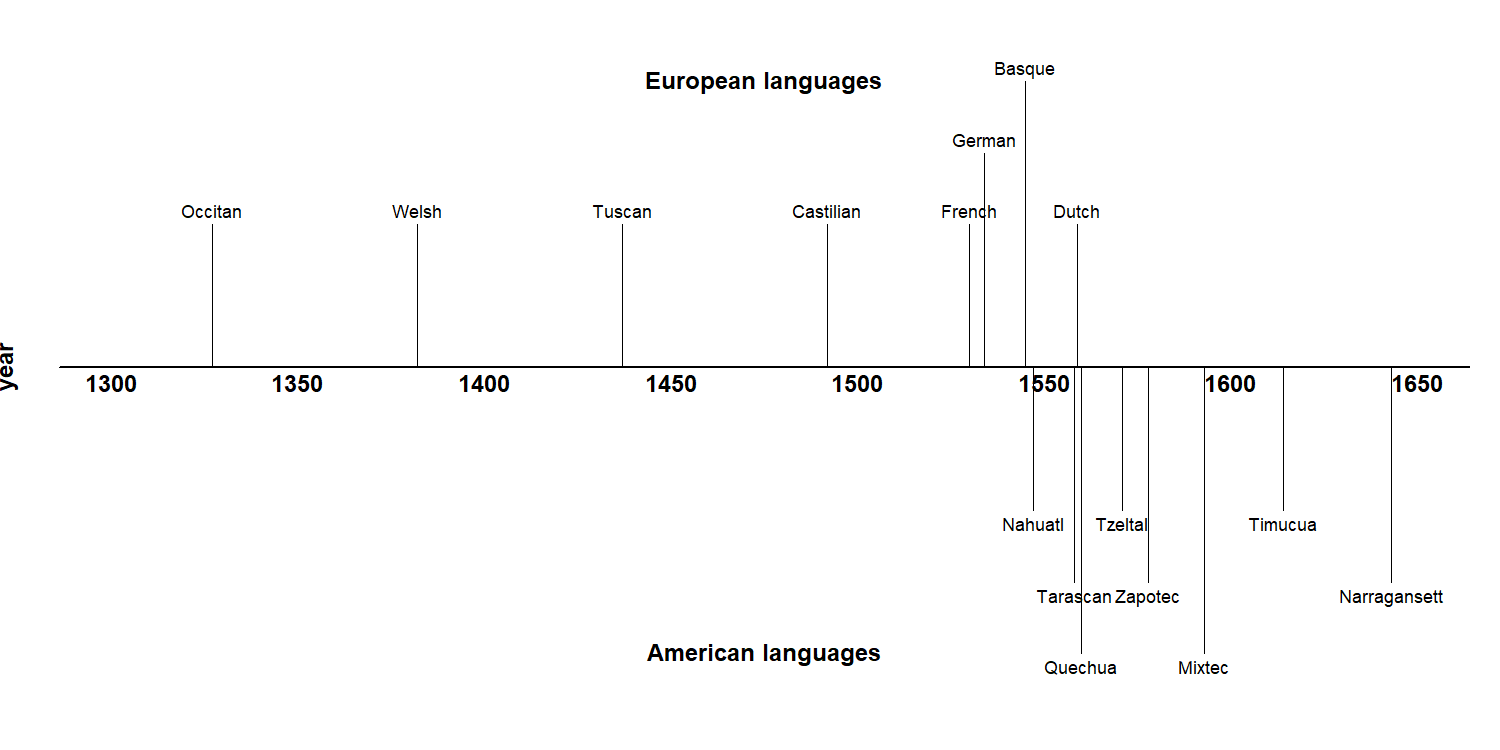
\includegraphics[width=\linewidth]{grammars.png}
  \caption{Approximate date of some of the first grammatical descriptions of European vs. American languages}
  \label{fig:grammars}
\end{figure}

\singlespacing
\setlength\LTleft{0pt}
\setlength\LTright{0pt}
\renewcommand{\arraystretch}{1.5}

\begin{longtable}[t]{ l l l l }%
  \caption{Some first grammatical descriptions of European vs. American languages}
  \label{tab:grammars}\\
  \toprule
    Language     & Year       & Title                                                                                                                                                                                         & Author\\
  \midrule
  \endfirsthead
  \caption[]{Some first grammatical descriptions of European vs. American languages}\\
  \toprule
    Language     & Year       & Title                                                                                                                                                                                         & Author\\
  \midrule
  \endhead
    \idx{Irish}        & 600s       & \parbox[t]{2.5in}{\pubtitle{Auraicept na n-Éces}\\\tln{The scholars' primer}}                                                                                                                 & Longarad\\
    \idx{Occitan}      & 1327       & \parbox[t]{2.5in}{\pubtitle{Leys d'amors}\\\tln{Laws of love}}                                                                                                                                & Guilhèm Molinièr\\
    \idx{Welsh}        & 1382--1410 & \parbox[t]{2.5in}{\pubtitle{Llyfr Coch Hergest}\\\tln{Red book of Hergest}}                                                                                                                   & unknown\\
    \idx{Tuscan}       & 1437--1441 & \parbox[t]{2.5in}{\pubtitle{Grammatica della lingua toscana}\\\tln{Grammar of the Tuscan language}}                                                                                           & Leon Battista Alberti\\
    Castilian\index{Spanish}    & 1492       & \parbox[t]{2.5in}{\pubtitle{Gramática de la lengua castellana}\\\tln{Grammar of the Castilian language}}                                                                                      & Antonio de Nebrija\\
    \idx{French}       & 1530       & \parbox[t]{2.5in}{\pubtitle{L'Éclaircissement de la langue francoyse}\\\tln{Explication of the French language}}                                                                              & John Palsgrave\\
    \idx{German}       & 1534       & \parbox[t]{2.5in}{\pubtitle{Ein Teutsche Grammatica}\\\tln{A German grammar}}                                                                                                                 & Valentin Ickelsamer\\
    \idx{Basque}       & 1545       & \parbox[t]{2.5in}{\pubtitle{Linguæ Vasconum Primitiæ}\\\tln{First fruits of the Basque language}}                                                                                             & Bernard Etxepare\\
    \idx{Totonac}      & 1539--1554 & \parbox[t]{2.5in}{\pubtitle{Arte de la lengua totonaca}\\\tln{Grammar of the Totonac language}}                                                                                               & Andrés de Olmos\\
    \idx{Nahuatl}      & 1547       & \parbox[t]{2.5in}{\pubtitle{Arte para aprender la lengua mexicana}\\\tln{Grammar for learning the Mexican language}}                                                                          & Andrés de Olmos\\
    \idx{Tarascan}     & 1558       & \parbox[t]{2.5in}{\pubtitle{Arte de la lengua tarasca de Michoacán}\\\tln{Grammar of the Tarascan language of Michoacán}}                                                                     & Maturino Gilberti\\
    \idx{Dutch}        & 1559       & \parbox[t]{2.5in}{\pubtitle{Den schat der Duytsscher Talen}\\\tln{The treasure of the Dutch language}}                                                                                        & John III van de Werve\\
    \idx{Quechua}      & 1560       & \parbox[t]{2.5in}{\pubtitle{Grammatica o arte de la lengua general de los Indios de los Reynos del Peru}\\\tln{Grammar or Art of the General Language of the Indians of the Royalty of Peru}} & Domingo de Santo Tomás\\
    \idx{Tzeltal Maya} & 1571       & \parbox[t]{2.5in}{\pubtitle{Ars Tzeldaica}\\\tln{Tzeltal Grammar}}                                                                                                                            & Fray Domingo de Hara\\
    \idx{Zapotec}      & 1578       & \parbox[t]{2.5in}{\pubtitle{Arte en lengua Zapoteca}\\\tln{Grammar in the Zapotec language}}                                                                                                  & Juan de Córdova\\
    \idx{English}      & 1586       & \parbox[t]{2.5in}{\pubtitle{Pamphlet for Grammar}}                                                                                                                                            & William Bullokar\\
    \idx{Mixtec}       & 1593       & \parbox[t]{2.5in}{\pubtitle{Arte de lengua Mixteca}\\\tln{Grammar of the Mixtec language}}                                                                                                    & Antonio de los Reyes\\
    \idx{Timucua}      & 1614       & \parbox[t]{2.5in}{\pubtitle{Gramatica de la lengua Timuquana de Florida}\\\tln{Grammar of the Timucua language of Florida}}                                                                   & Francisco Pareja\\
    \idx{Narragansett} & 1643       & \parbox[t]{2.5in}{\pubtitle{A key into the language of America}}                                                                                                                              & Roger Williams\\
  \bottomrule
\end{longtable}

\renewcommand{\arraystretch}{1}
\doublespacing

As documentary linguistics turned its attention to North American (as opposed to Mesoamerican) languages, lexical flexibility in particular became a more prominent issue. In fact, even the first comprehensive survey of North American languages contains an entire section on \enquote{Conversion of nouns into verbs} \parencite[174--177]{Gallatin1836}, in which Gallatin depicts lexical flexibility as a rampant feature of all languages on the continent:

\blockquote[{\cite[175--176]{Gallatin1836}}]{It is the substantive [i.e. copula / auxiliary] verb which we [speakers of Indo-European languages] conjugate; whilst the [Native American] conjugates what we call the adjective and even the noun itself, in the same manner as [s/he] does other intransitive verbs. […] I believe it must appear sufficiently obvious, that this general if not universal character of the [Native American] languages, the conversion into verbs and the conjugation, through all the persons, tense, and moods, of almost all the adjectives and of every noun which, without a palpable absurdity, is suspectible of it, is entirely due to the absence of the substantive verb.}

As evidenced by the above passage, increasing familiarity with non-\idx{Indo-European} languages prompted some writers to abandon the universalist commitment. However, categorial universalism is still a widely-held position today, either in the sense of a) being universally instantiated in all languages \parentext{commonly assumed by most generative frameworks; although see \textcite{Culicover1999}}, or b) being available to all languages, but only instantiated in some \parentext{sometimes called the \enquote{smörgåsbord} or \enquote{grab bag} approach, as exemplified by \citeauthor{Dixon2010}'s Basic Linguistic Theory framework \parencites*[9, 11, 14, 27, 50]{Dixon2010}[26]{Dixon2011}; \textcite[298]{Hieber2013}; \textcite[10]{Croft2001b}}.

\subsection{Relativism}
\label{sec:2.2.2}

American ethnographers in the tradition of Franz Boas questioned the univeralist assumption in a programmatic and comprehensive way. Writing on grammatical categories, \citeauthor{Boas1911} states, \textquote[{\cite[35]{Boas1911}}]{Grammarians who have studied the languages of Europe and western Asia have developed a system of categories which we are inclined to look for in every language}. He concludes that this endeavor is a folly, and that \textquote[{\cite[35]{Boas1911}}]{in a discussion of the characteristics of various languages \qem{different fundamental categories} will be found}. Boas' students all adopted his grammatical relativism, and it became a foundational principle of the American linguistics tradition. His student Edward Sapir, writing on lexical categories specifically, makes one of the best-known and strongest statements of this position in his influential textbook \pubtitle{Language}: \textquote[{\cite[125]{Sapir1921}}]{[N]o logical scheme of the parts of speech—their number, nature, and necessary confines—is of the slightest interest to the linguist. Each language has its own scheme. Everything depends on the formal demarcations which it recognizes.}.

Many linguists today hold to Boas' grammatical relativism in some fashion or another. Textbooks and typological surveys commonly state that languages have varying numbers of lexical categories, though usually with the caveat that all languages seem to differentiate at least noun and noun \parencite[e.g.][§6.2]{Velupillai2012}. Some researchers, especially those working in typology, argue that linguists are still not rigorous \emph{enough} in their application of grammatical relativism; they criticize certain kinds of crosslinguistic comparisons for imposing the categories of one language onto another \parencites{Croft2001b}{Gil2001}{Haspelmath2010a}{Haspelmath2012}{LaPolla2016}. This position is discussed further in \secref{sec:2.4}.

\subsection{Structuralism}
\label{sec:2.2.3}

Developing alongside the early anthropological linguistics of Boas was the linguistic structuralism of Ferdinand de Saussure. His work informed both the Prague school under Nikolay Trubetzkoy and Roman Jakobson, and the distributional method of Leonard Bloomfield. The term \dfn{structuralism} has any number of uses \parencite[Ch.~1]{Matthews2001}; here I refer to the idea that \textquote[{\cite[383]{Matthews2014}}]{language is a […] self-contained, self-regulating system, whose elements are defined by their relationship to other elements}. In particular, I am referring to the positivistic flavor of structuralism as practiced by Bloomfield, which focused on the structural relations between elements and establishing a set of rigorous scientific discovery procedures for linguistic structures \parencite{Bloomfield1933}. Bloomfield saw lexical categories as something to be empirically discovered in the different syntactic distributions of words, rather than imposed on a language a priori \parencite[33]{Rauh2010}. Zellig Harris later refined and expanded on this methodology \parencite{Harris1951}, which in turn was incorporated into Noam Chomsky's ealy Phrase Structure Grammar.

The signature methodological feature of this form of structuralism is the \dfn{distributional method}, a procedure for defining categories in terms of the set of contexts in which its words can appear—that is, their distributions \parencites[5]{Harris1951}[11]{Croft2001b}. As an illustration of distributional analysis applied to lexical categories, \textcite[11--12]{Croft1991} considers the distributions of the \idx{English} words \txn{cold}, \txn{happy}, \txn{dance}, and \txn{sing} in two constructions: in the Predicate construction after \txn{be}, and in the \nth{3} Person Singular Present Tense (\txn{-s}) construction. Example data are shown below.

\begin{exe}
  \ex\label{ex:2.2}
  \exinfo{\idx{English} (Indo-European > Germanic)}
  \begin{xlist}
    \ex
      \begin{xlist}
        \setlength{\itemsep}{0em}
        \ex[]{Jack is cold.}
        \ex[*]{Jack colds.}
      \end{xlist}
    \ex
      \begin{xlist}
        \setlength{\itemsep}{0em}
        \ex[]{Jack is happy.}
        \ex[*]{Jack happies.}
      \end{xlist}
    \ex
      \begin{xlist}
        \setlength{\itemsep}{0em}
        \ex[*]{Jack is dance.}
        \ex[]{Jack dances.}
      \end{xlist}
    \ex
      \begin{xlist}
        \setlength{\itemsep}{0em}
        \ex[*]{Jack is sing.}
        \ex[]{Jack sings.}
      \end{xlist}
  \end{xlist}
\end{exe}

We can see that \txn{cold} and \txn{happy} have the same distributions in these tests (both may appear in the Predicate construction but not the Person-Tense inflection construction), while \txn{dance} and \txn{sing} have the same distribution (the inverse situation as \txn{cold} and \txn{happy}). The results of these two distributional tests are summarized in \tabref{tab:English-distributions-a}.

\begin{table}[h]
  \centering
  \caption[Distribution of \idx{English} Verbs and Adjectives]{Distribution of English Verbs and Adjectives \parentext{adapted from \textcite[12]{Croft2001b}}}
  \label{tab:English-distributions-a}
  \begin{tabular}{ l c c }
    \toprule
    { } & \parbox{1in}{\centering Predicate{\newline}Construction} & \parbox{1in}{\centering Inflectional{\newline}Construction}\\
    \midrule
    \textbf{Adjective}: \txn{cold}, \txn{happy}, etc. & ✔ & ✘\\
    \textbf{Verb}:      \txn{sing}, \txn{dance}, etc. & ✘ & ✔\\
    \bottomrule
  \end{tabular}
\end{table}

As applied in practice, however, the distributional method suffers from one serious drawback when used to argue for large, traditional categories like noun, verb, and adjective: distributional tests yield conflicting and overlapping results. Perhaps no two lexical items behave the same in every distributional test. Each new test that is introduced therefore partitions the lexicon into smaller and smaller classes. This fact has been demonstrated empirically for \idx{English} temporal nouns \parencite[54]{Crystal1967}, \idx{Russian} numerals \parencite{Corbett1978}, and \idx{French} verbs \parencite{Gross1979}. Distributional tables like that in \tabref{tab:English-distributions-a} from each of these studies are reproduced in \tabref{tab:French-distributions}, \tabref{tab:Russian-distributions}, and \tabref{tab:English-distributions-b} respectively. It is clear from these studies that distributional analysis does \emph{not} lead to large, unified categories like noun, verb, and adjective, but rather a myriad of small constructions \parencites[27]{Crystal1967}[434]{Croft2005}. Each distributional test is in fact its own construction \parencite[436]{Croft2005}. This fact is the motivation underlying constructional approaches to language.

\begin{figure}[h!]
  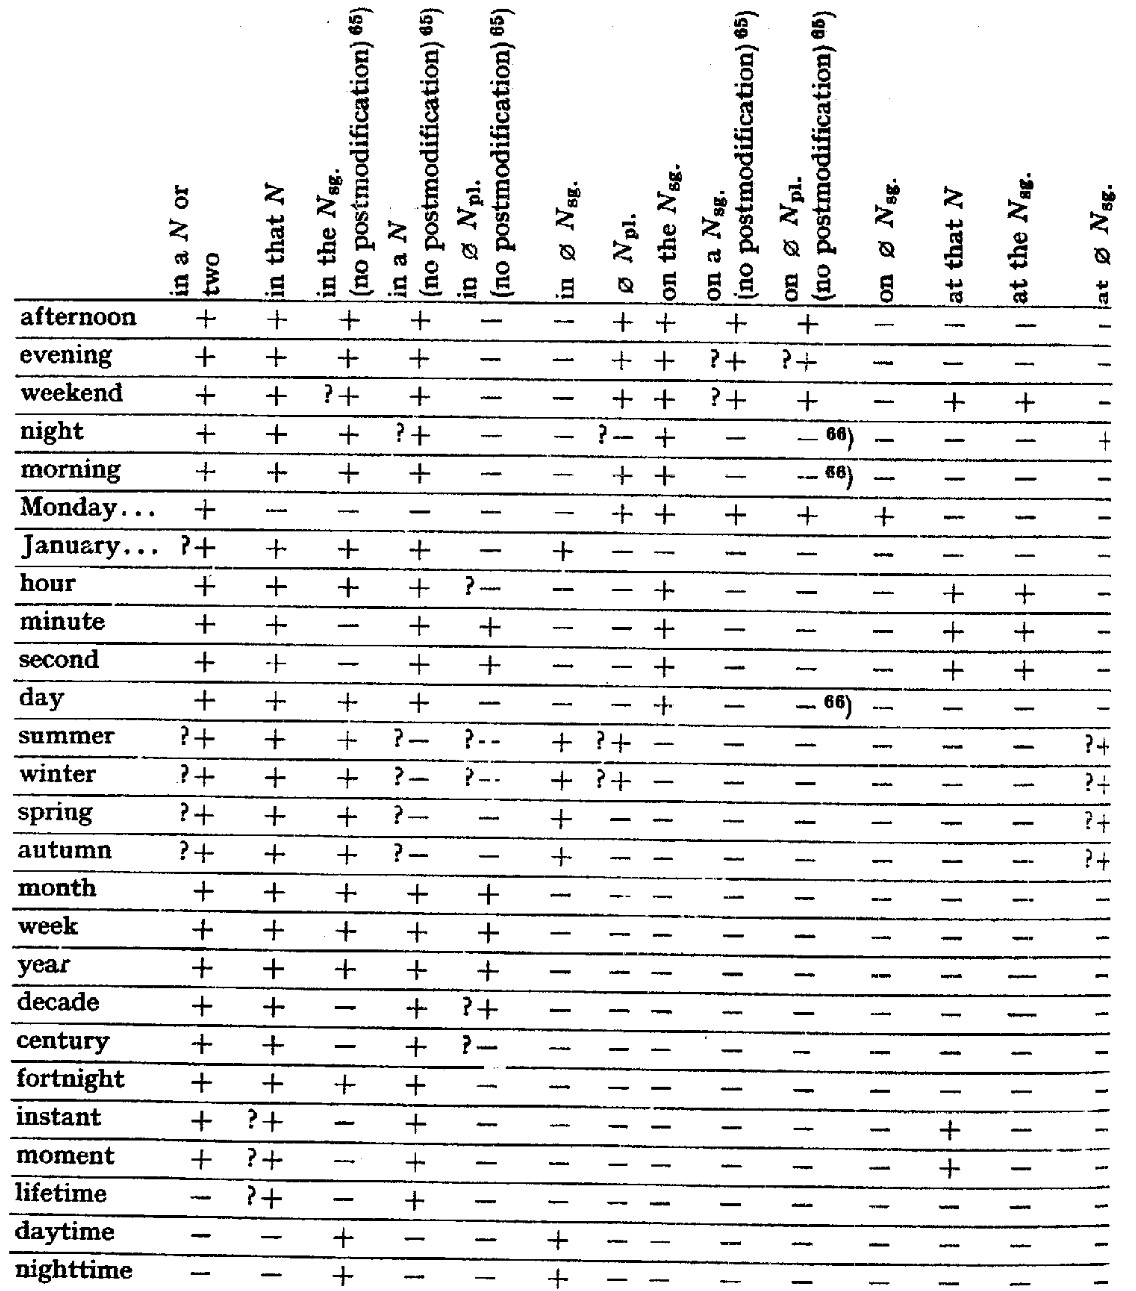
\includegraphics[width=\linewidth]{English-distributions.jpg}
  \caption[distributional analysis of English temporal nouns]{distributional analysis of \idx{English} temporal nouns \parencite[54]{Crystal1967}}
  \label{fig:English-distributions-b}
\end{figure}

\begin{figure}[h!]
  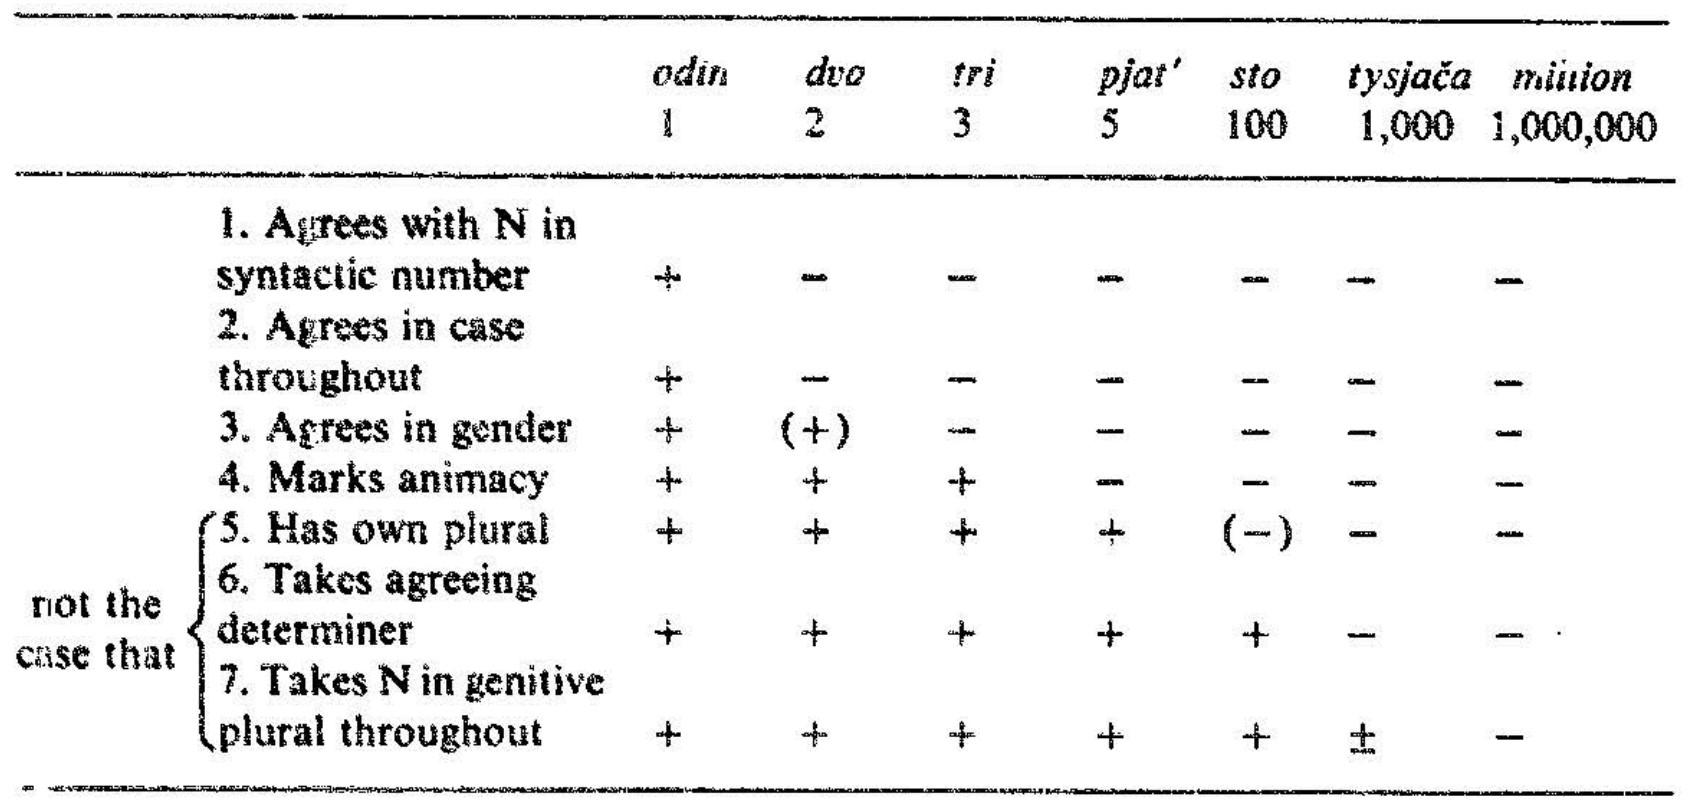
\includegraphics[width=\linewidth]{Russian-distributions.jpg}
  \caption[distributional analysis of Russian numerals]{distributional analysis of \idx{Russian} numerals \parencite[359]{Corbett1978}}
  \label{fig:Russian-distributions}
\end{figure}

\begin{figure}[h!]
  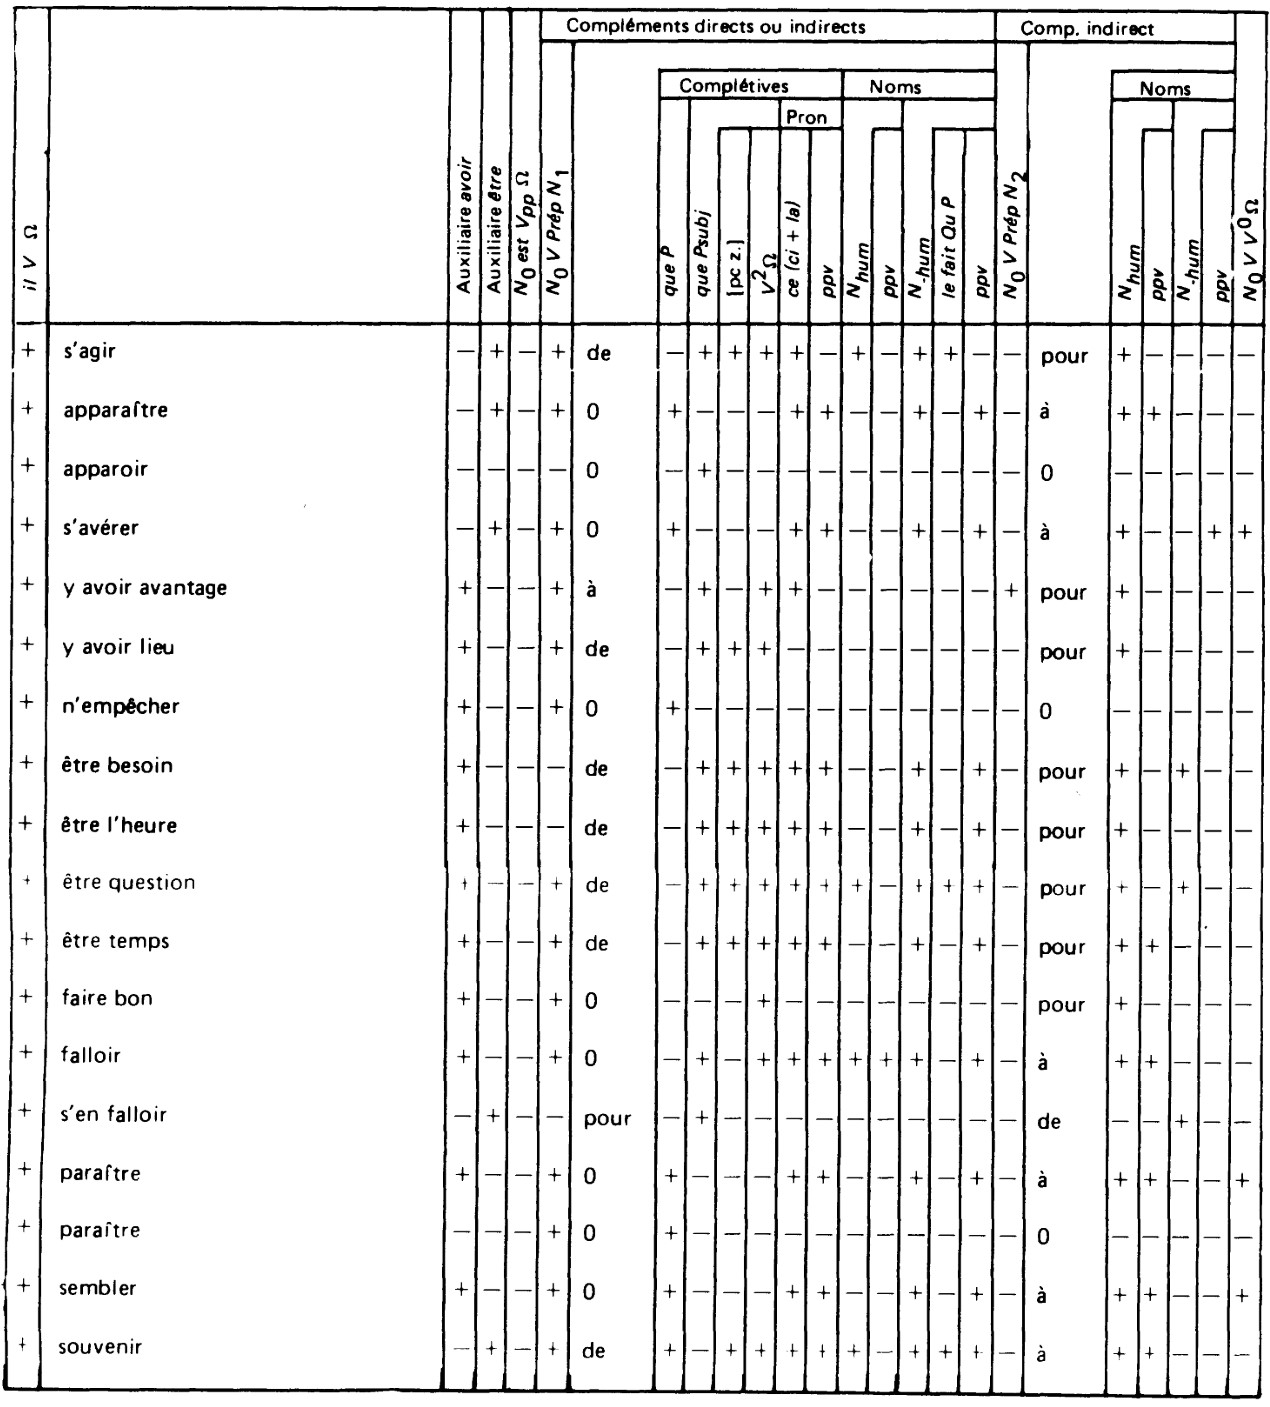
\includegraphics[width=\linewidth]{French-distributions.jpg}
  \caption[distributional analysis of French verbs]{distributional analysis of \idx{French} verbs \parencite[860]{Gross1979}}
  \label{fig:French-distributions}
\end{figure}

Many scholars nonetheless choose to retain lexical categories as a necessary component of their linguistic theories or descriptions, at the expense of consistent application of the distributional method. Rather than considering all possible distributional contexts for a word, these scholars instead treat certain constructions as definitional of the category. Other distributional tests which yield cross-cutting results are either ignored, or treated as evidence of subcategories instead of categories. Many researchers even prefer the term \dfn{syntactic categories} over \dfn{lexical categories} for this reason, focusing on just the syntactic evidence for categories \parencites{Baker2003}{Rauh2010}. A severe methodological problem for this approach is that there are no generally agreed-upon principles for determining which distributional tests should be considered definitional. In this regard, \textcite[4]{SchachterShopen2007} note, \textquote{there may be considerable arbitrariness in the identification of distinct parts of speech rather than subclasses} \parentext{see also \textcite{Crystal1967}}. Different scholars choose or prioritize different kinds of evidence for lexical categories over others on the basis of their theoretical commitments. This is the reason, as stated in \secref*{sec:1.1}, that disagreements about the existence of particular lexical categories in particular languages are typically \emph{not} about the empirical facts. The results of a given distributional analysis are not usually controversial; the choice of distributional tests used to support one's analysis are. Unsurprisingly, then, debates over how to analyze lexical categories in various languages have been largely unproductive and unresolved \parencite[435]{Croft2005}. The problem only worsens when scholars attempt to apply the same criteria across languages. Distributions of words with similar meanings vary drastically across languages \parencite[§1.4.1]{Croft2001b}.

The real methodological problem here is \emph{not} that we have yet to ascertain the correct principles for selecting the right distributional tests. The problem is being selective regarding which tests to apply in the first place. If we take the distributional method seriously, then we must apply it consistently, without ignoring distributional evidence that contradicts our theoretical or pretheoretical assumptions. To do otherwise is a kind of \dfn{methodological opportunism} \parencite[30, 41]{Croft2001b}.

Other scholars treat flexible words as members of \dfn{hybrid} or \dfn{mixed} categories simultaneously possessing properties of more than one part of speech \parencites[149]{Loisetal2017}{Malouf1998}{NikolaevaSpencer2020}. Adjectives are frequently described as a hybrid category \parencites{Wetzer1996}[343]{Stassen1997}[13--16]{Pustet2003}[95]{GenettiHildebrandt2004}{Lier2017}, as are participles \parencite[704]{HopperThompson1984} and gerunds \parencite{Denison2001}. \textcite[149]{Loisetal2017} distinguish hybridity from polycategoriality, stating that polycategoriality applies to roots or stems, while hybridity is a matter of the syntactic context that a word appears in.

An analysis couched in mixed categories does not avoid the problem of methodological opportunism, however. The existence of a mixed category implies that there are other, more basic categories that the mixed category is a hybrid of. Hybrid models of parts of speech merely exacerbate the distributional problem. There is however a sense in which viewing minor lexical categories as mixed categories is useful, and that is when one views lexical categories as typological markedness patterns arising from combinations of the semantic classes of object, action, or property words with the discourse functions of reference, predication, and modification. Categories frequently discussed as \enquote{mixed} are precisely those combinations which are non-prototypical and therefore more likely to be typologically marked. \secref*{sec:2.4.2} explains this approach to lexical categories in more detail.

Partly in response to these problems, a growing cadre of linguists in the last 30 years have adopted one of various \dfn{flexible} approaches to word classes. Flexible analyses of word classes come in many flavors, some of which arguably still commit methodological opportunism, and others of which introduce new difficulties. These flexible approaches are reviewed in the following section.

\section{Flexible approaches}
\label{sec:2.3}

In this section I summarize the key concepts (\secref{sec:2.3.1}), findings (\secref{sec:2.3.2}), and criticisms (\secref{sec:2.3.2}) of lexical flexibility research. \secref*{sec:2.3.1} surveys the wide variety of definitions and theoretical perspectives on lexical flexibility. This review of the literature reveals that there is very little consensus as to what exactly constitutes \enquote{lexical flexibility}; as such, there are numerous alternative terms for the phenomenon. Despite these incongruities, a few important findings do consistently surface across the empirical research. These findings are summarized in \secref*{sec:2.3.2}. \secref*{sec:2.3.3} then looks at the arguments and evidence that researchers have presented against the notion of lexical flexibility.

\subsection{Key concepts}
\label{sec:2.3.1}

It is only a small exaggeration to say that there are as many definitions and terms for what I am here calling \enquote{lexical flexibility} as there are scholars who research it. I use the term \dfn{lexical flexibility} in this thesis merely because it is the most widely recognized of the cluster of terms that are used, not because it is necessarily the most precise or accurate. My own choice would be \dfn{functional expansion}, for reasons discussed below. The analytical or theoretical perspective adopted by each researcher generally determines their choice of terminology. The remainder of this section is devoted to explaining these perspectives in more detail.

Generally speaking, there are two ways to analyze flexible words. The first method assigns flexible words to members of specific categories in a language, whether those language-categories are the canonical four major classes (Noun, Verb, Adjective, Adverb), or a new large supercategory subsuming multiple discourse functions (e.g. contentives, non-verbs, flexibles), or a smaller subcategory of an existing major lexical category (e.g. adjective verbs, verbonominals). The second method of analysis assumes that words are uncategorized at some level (root, stem, or inflected word), and that words receive their categorial assignment from context. Different researchers posit different mechanisms for how words receive their categorization in context. The traditional approaches to lexical flexibility summarized in \secref*{sec:2.2} are all instances of the former method of analysis, while the flexible approaches outlined in this section are a mix of categorial and non-categorial analyses.

\subsubsection{Lexical flexibility}
\label{sec:2.3.1.1}

Though awareness of lexical flexibility can be traced back to at least \textcite[174--177]{Gallatin1836} if not earlier, the term \dfn{lexical flexibility} itself seems to have originated with \textcite[Ch.~4]{Hengeveld1992}. This publication, perhaps because it was the first to assign a technical term to the concept, marks a shift in how scholars frame the concept of lexical flexibility. Previously, the issue was framed in terms of whether particular languages (especially those of the Pacific Northwest) distinguished noun from verb \parencites{Kuipers1968}{Jacobsen1979}{Hebert1983}{Kinkade1983}{EijkHess1986}{JelinekDemers1994}. After this point, an increasing number of publications began to ask whether lexemes were \dfn{flexible} instead. Though the difference in emphasis seems subtle, this change constitutes a turning point because it fostered an increased interest in lexical flexibility as a grammatical phenomenon in its own right instead of just a problem for traditional categorization schemes.

\citeauthor{Hengeveld1992}'s \citeyear[Ch.~4]{Hengeveld1992} typology of parts-of-speech systems is a whole-language typology wherein languages are either \dfn{specialized}, with one morphosyntactic category for each of the functions of reference (Noun), predication (Verb), referent modification (Adjective), and predicate modification (Adverb\footnote{Note that Hengeveld's typology only includes manner adverbs, not other semantic types of adverbs.}), or \dfn{non-specialized}. Non-specialized languages deviate from the four-category canon in one of two ways: one part of speech may assume more than one function with no additional morphosyntactic marking, in which case the language is considered \dfn{flexible}; or the language may lack a dedicated part of speech for that function entirely and use other, marked constructions instead, in which case the language is considered \dfn{rigid}.

\citeauthor{Hengeveld1992} gives examples from \idx{Dutch} and \idx{Wambon} to illustrate the distinction between rigid and flexible languages. In the Dutch examples in \exref{ex:2.3}, the same word \txn{mooi} is used for both referent modification \exref{ex:2.3a} and predicate modification \exref{ex:2.3b}, with no overt morphology indicating its function in either case. Wambon on the other hand uses medial verbs for manner expressions, and must take the overt verbalizing suffix \txn{-mo} shown in \exref{ex:2.4}. In \citeauthor{Hengeveld1992}'s framework, Dutch is a flexible language because one category subsumes both the functions of referent modification and predicate modification, while Wambon is a rigid language because derivational morphology (here, the verbalizing suffix \txn{-mo}) is required to indicate the function of predicate modification.

\begin{exe}

  \ex\label{ex:2.3}
  \exinfo{\idx{Dutch} (Indo-European > Germanic)}
  \begin{xlist}

    \ex\label{ex:2.3a}
    \gll een        \em{mooi}      kind\\
         \gl{indef} \em{beautiful} child\\
    \tln{a beautiful child}
    \exsource[65]{Hengeveld1992}

    \ex\label{ex:2.3b}
    \gll het      kind  dans‑t              \em{mooi}\\
         \gl{def} child dance‑\gl{3sg.pres} \em{beautifully}\\
    \tln{the child dances beautifully}
    \exsource[65]{Hengeveld1992}

  \end{xlist}

  \ex\label{ex:2.4}
  \exinfo{\idx{Wambon} (Trans-New Guinea > Greater Awyu)}
  \gll jakhov‑e       \em{matet‑mo}         ka-lembo\\
       they‑\gl{conn} \em{good‑\gl{vzr.ss}} go‑\gl{3pl.past}\\
  \tln{did they travel well?}
  \hfill\hspace*{1em}\mbox{\footnotesize\parentext{\textcite[49]{Vries1989}, cited in \textcite[65]{Hengeveld1992}}\normalsize}

\end{exe}

\citeauthor{Hengeveld1992}'s analysis is of the categorial type discussed at the beginning of \secref*{sec:2.3.1}, specifically the supercategory kind. Each word is assumed to have a category, and new supercategories are introduced for words which have multiple functions: \dfn{contentives} for words which perform all four functions, \dfn{non-verbs} for words which perform all non-predicating functions, and \dfn{modifiers} for words which perform referent modifier and predicate modifier functions.

\citeauthor{Hengeveld1992}'s parts-of-speech typology and the subsequent research it inspired \parencites{DonLier2003}{HengeveldRijkhoff2005}{Lier2006}{HengeveldLier2010}{Luuk2010}{LierRijkhoff2013}{Lier2016} constitute important empirical contributions to the study of lexical flexibility. However, Hengeveld's definition of flexible languages and his parts-of-speech typology still rely on large, language-specific categories of the kind that have been problematized by \textcite[§2.2.2]{Croft2001b} and \textcite{CroftLier2012}, and are therefore subject to the same difficulties as traditional approaches to parts of speech. However, numerous scholars have since adopted Hengeveld's term \dfn{lexical flexibility} to describe cases where words serve more than one discourse function, regardless of their particular theoretical commitments or analysis of flexible words. As a convenient cover term, \dfn{lexical flexibility} is now well established.

\subsubsection{Polycategoriality}
\label{sec:2.3.1.2}

\textcite[4]{VapnarksyVeneziano2017} introduce the alternative term \dfn{polycategoriality} as their preferred characteriziation of flexible words. (The term is also used by \textcite{Carter2006}, but he does not give a precise definition for it.) While \citeauthor{VapnarksyVeneziano2017} use this term mostly interchangeably with \dfn{lexical flexibility}, there are important differences between the two concepts. \citeauthor{Hengeveld1992}'s use of \dfn{lexical flexibility} is meant to imply the existence of large, flexible supercategories that subsume multiple discourse functions, whereas Vapnarksy \& Veneziano are not committed to any particular schema for parts of speech. Central to their notion of polycategoriality is the idea that lexical categories exist, but that \textquote[{\cite[4]{VapnarksyVeneziano2017}}]{there are lexical forms that are not specified for lexical category (or are not specified fully, or univocally) on some level of representation.}. In other words, one word may belong simultaneously to multiple lexical categories. Under this definition, a language could still have all four major lexical categories but nonetheless exhibit rampant polycategoriality; this is not a possibility in \citeauthor{Hengeveld1992}'s framework. Like \citeauthor{Hengeveld1992}, however, \citeauthor{VapnarksyVeneziano2017} are committed to the existence of large lexical categories in particular languages. Their analysis is therefore also of the categorial kind discussed at the beginning of \secref*{sec:2.3.1}.

\subsubsection{Multifunctionality / Polyfunctionality}
\label{sec:2.3.1.3}

Another term for our phenomenon of interest, introduced by \parencite{Lier2012}, is \dfn{multifunctionality}, in which a single lexeme can have multiple discourse functions. An advantage of this analysis is that it takes no theoretical position on the issue of whether words are categorial or acategorial; it focuses on just their functions. The term \dfn{multifunctionality} is meant to stand in contrast with \dfn{conversion} or \dfn{zero derivation}. \citeauthor{Lier2012} takes conversion to be idiosyncratic and unproductive, producing meanings for words in alternate discourse functions that are not predictable (see \secref{sec:2.3.2.4} and \secref{sec:2.3.3.2} for further discussion). Multifunctionality is also distinct from zero derivation from a common root. Instead, multifunctional words are those whose semantic interpretation is entirely predictable from context, and its uses in different contexts are productive. Its meaning should be \dfn{compositional}. For example: when an action word is used in a referring construction its predicted meaning is that of an \dfn{action nominalization}, \tln{(the act of) X‑ing}; and when an object word is used in a predicate construction its predicted meaning is that of a \dfn{predicate nominal}, \tln{be an X}. Examples of these predictable, compositional meanings for flexible words in \idx{Chamorro} are shown in \exref{ex:2.5}.

\begin{exe}

  \ex\label{ex:2.5}
  \exinfo{\idx{Chamorro} (Austronesian > Malayo-Polynesian)}
  \begin{xlist}

    \ex\label{ex:2.5a}
    \gll para     \em{batångga‑n}     karabåo esti\\
         \gl{fut} \em{shed‑\gl{link}} carabao this\\
    \tln{this is going to be a carabao shed}
    \exsource[8]{Chung2012}

    \ex\label{ex:2.5b}
    \gll para     \em{gatbesa}    ha'\\
         \gl{fut} \em{decoration} \gl{emph}\\
    \tln{[she] is going to be a decoration}
    \exsource[20]{Chung2012}

  \end{xlist}

\end{exe}

\noindent In the two examples above, the meaning of the object words \tln{shed} and \tln{decoration} are predictable when used in a predicative context: \tln{be a shed/decoration}. However, words used in their non-prototypical functions very frequently do not have predictable meanings. Consider the example in \exref{ex:2.6}.

\begin{exe}
  \ex\label{ex:2.6}
  \exinfo{\idx{Chamorro} (Austronesian > Malayo-Polynesian)}
  \gll ma       \em{se'si'} i   babui\\
       \gl{agr} \em{knife}  the pig\\
  \tln{they stabbed the pig}
  \exsource[29]{Chung2012}
\end{exe}

\noindent In this example, the meaning \tln{stab} cannot be predicted from the meaning of the object word \tln{knife}. It could have just as easily meant \tln{be a knife} or \tln{cut}.

\citeauthor{Lier2012} takes examples like those in \exref{ex:2.5} to be instances of genuine multifunctionality, and those in \exref{ex:2.6} to be cases of conversion. Others have also adopted a position similar to \citeauthor{Lier2012}'s, in which only the semantically compositional / predictable uses of a word in different discourse functions are considered flexible \parencites[§2.2.2--§2.2.3]{Croft2001b}[§3.2]{EvansOsada2005}.

\subsubsection{Precategoriality / Acategoriality}
\label{sec:2.3.1.4}

The various approaches which analyze flexible words as being at some level uncategorized until they receive their interpretation from context may be lumped together under the umbrella terms \dfn{precategoriality} or \dfn{acategoriality}. \citeauthor{HopperThompson1984}'s influential paper \citeyear{HopperThompson1984} is an early application of the concept of acategoriality to the analysis of flexible words:

\blockquote[{\cite[747]{HopperThompson1984}}]{[L]inguistic forms are in principle to be considered as \emph{lacking categoriality} completely unless nounhood or verbhood is forced on them by their discourse functions. To the extent that forms can be said to have an apriori existence outside of discourse, they are characterizable as \dfn{acategorial}; i.e. their categorical classification is irrelevant. Categoriality-the realization of a form as either a N or a V-is imposed on the form by discourse.}

The term \dfn{precategorial} has become a somewhat more common term for roughly the same concept (though some researchers use the term in more strictly-delineated ways) \parencites[357, 362--364]{EvansOsada2005}{Bisang2008}{Bisang2013}. It is especially preferred by morphological models that presuppose stages of derivation, such that words are precategorial before they reach a certain stage of the derivation \parencites{HalleMarantz1994}{Arad2005}{McGinnisArchibald2016}{Siddiqi2018}. \textcite[5]{VapnarksyVeneziano2017} distinguish polycategoriality from acategoriality by defining acategoriality as implying \textquote{no primitive / original categorial marking at all}, and polycategoriality as allowing a form \textquote{to be only partially unspecified for category, with possible constraints on the relevant categories}. Languages for which precategorial analyses have been advanced include \idx{Cherokee} \parencite{Haag2017}, \idx{Gooniyandi} \parencite{McGregor2013}, \idx{Kuikuro} \parencite{FranchettoSantos2017}, Mundari \parencite{HengeveldRijkhoff2005}, and many others. \textcite{Pfeiler2006} also presents pscyholinguistic evidence that the earliest utterances of L1 learners of \idx{Yucatec Maya} are acategorial.

A central concern in precategorial approaches is the precise mechanism by which a word receives its categorization in context \parencite[§3.7]{HengeveldRijkhoffSiewierska2004}. There are two main theories of semantic indeterminacy in flexible words: \dfn{underspecificity} \parencites{Farrell2001}{RijkhoffLier2013} and \dfn{vagueness} \parencites{Tuggy1993}{HengeveldRijkhoffSiewierska2004}{HengeveldRijkhoff2005}. The essential difference is that underspecificity entails semantic minimalism while vagueness is entails semantic maximalism. An underspecified word has a minimal, core meaning, and receives its categorial meaning from the discourse context it appears in; a vague word has a maximal, broad meaning that covers all the possible discourse contexts it appears in. (There is of course quite a deal of variation in the literature as to how scholars use these terms, with many researchers conflating the two.) \textcite[414]{HengeveldRijkhoff2005} offer the example of \idx{English} \txn{cousin} as a word that is semantically underspecified for gender, such that the gender of the referent must be understood from context. \textcite{Denison2018} argues that the English word \txn{long} exhibits adjective {\textasciitilde} adverb underspecification in \idx{Old English} and \idx{Middle English}.

In contrast, \textcite[539--541]{HengeveldRijkhoffSiewierska2004} outline a theory regarding exactly how vagueness operates in the context of lexical flexibility:

\blockquote[{\cite[541]{HengeveldRijkhoff2005}}]{[E]ach flexible lexeme has a single (vague) sense. By placing the flexible lexeme in a particular syntactic slot or by providing it with certain morphological markers, the speaker highlights those meaning components of the flexible lexeme that are relevant for a certain lexical (verbal, nominal, etc.) function. Thus we contend that the meaning of a flexible lexeme always remains the same, and that morphosyntactic and other contextual clues signal to the addressee how to interpret this lexeme in an actual utterance. In other words, it is the use of a vague lexeme in a certain context (an actual linguistic expression) that brings out certain parts of its meaning, giving the category-neutral lexeme a particular categorial (verbal, nominal, etc.) flavour.}

\noindent (Note that while vagueness implies a certain potential ambiguity, Hengeveld \& Rijkhoff reserve the term \dfn{ambiguity} for cases of distinct, homophonous words.)

\textcite[363--364]{EvansOsada2005} and \textcite{Kihm2017} criticize both precategorial approaches for their imprecision, claiming that it would be impossible to formulate a definition for many flexible words that was broad enough to encompass all their uses. \textcite[87]{Kihm2017} illustrates this difficulty with the various meanings of the \idx{Arabic} root \txn{s-q-t}, which could arguably be glossed \textsc{fall}. A selection of stems containing this root are given in \exref{ex:2.7}.

\begin{exe}
  \ex\label{ex:2.7}
  \hspace{0.5em}\exinfo{\idx{Standard Arabic} (Afroasiatic > Semitic)}\\
  \begin{tabular}[t]{ p{0.75in} l }
    saqata   & \tln{to fall}\\
    saqiit   & \tln{hail}\\
    saqqaata & \tln{door latch}\\
    masqat   & \tln{place where a falling object lands; waterfall}\\
    isqaat   & \tln{overthrow; shooting down; miscarriage; substraction}\\
    tasaaqut & \tln{fall of hair}\\
    saaqita  & \tln{fallen woman; harlot}\\
    suquut   & \tln{fall; crash; collapse}\\
    saqt     & \tln{dew}\\
    siqt     & \tln{miscarried fetus}\\
    suqt     & \tln{sparks flying from a flint}\\
    saqat    & \tln{offal; rubbish}\\
    saqta    & \tln{tumble; slip; mistake}\\
    saaqit   & \tln{fallen; mean; missing}\\
  \end{tabular}
\end{exe}

It is difficult to imagine a single definition of \txn{s-q-t} which could adequately demarcate just this set of meanings. This difficulty could perhaps be overcome, however, by loosening the requirement that the meaning of a word be unitary. Word meanings are \dfn{polycentric}, where different senses of a word are related through \dfn{meaning chains} rather than all through a single, central member \parencite[110]{Taylor2003}. This is sometimes referred to as a \dfn{family resemblance} structure for categories. The difference between monocentric and polycentric categories is illustrated schematically in \figref{fig:family-resemblance}. In both diagrams, each letter A–E represents a sense of a word. In the monocentric case, all the senses of the word are related through its core sense A. In the polycentric case, senses A and E are related only through their intervening connections.

\begin{figure}[h!]
  \centering
  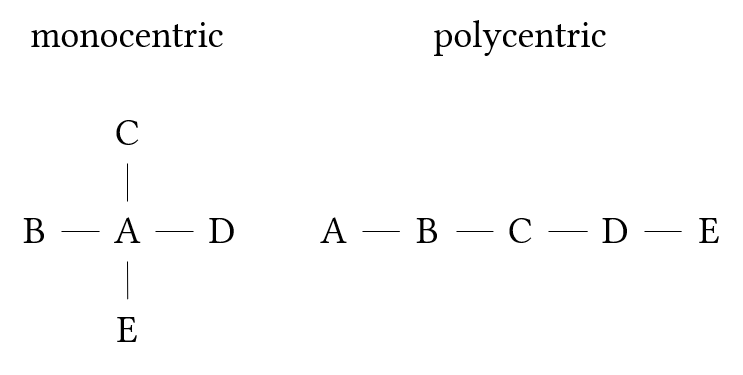
\includegraphics{monocentric-vs-polycentric.png}
  \caption{Monocentric versus polycentric categories}
  \label{fig:monocentric-vs-polycentric}
\end{figure}

Recognizing that word meanings are polycentric addresses \citeauthor{EvansOsada2005} and \citeauthor{Kihm2017}'s criticisms of vagueness theory because it shows that the disparate senses of a word can be related without having to share any core component of their meanings. The use of a lexeme in a certain context then profiles one of these senses over others. Kihm himself hints at this solution by referring to the related \idx{Arabic} stems in \exref{ex:2.7} as a \dfn{lexical family}.

\subsubsection{Monocategoriality}
\label{sec:2.3.1.5}

In the extreme case where all lexical words in a language are precatgorial, the language could be considered \dfn{monocategorial}, possessing a single, open syntactic category. This is effectively the same as saying that the language lacks lexical categories altogether, the difference being primarily one of emphasis. David Gil analyzes both \idx{Tagalog} \parencites*{Gil1993}{Gil1995} and Riau \idx{Indonesian} \parencite*{Gil1994} as being of this extreme monocategorial type. Moreover, he argues that monocategoriality must have been typical of an earlier stage of language evolution in which dedicated morphosyntactic constructions for different discourse functions had yet to evolve \parencites{Gil2005}{Gil2006}{Gil2012}. He names this abstract language type an \dfn{Isolating-Monocategorial-Associational} (IMA) language.

\subsubsection{Transcategoriality}
\label{sec:2.3.1.6}

It is also worth briefly mentioning \dfn{transcategoriality}, since the term arises occasionally in connection with lexical flexibility and is potentially easily confused with other terms mentioned above. \textcite{Robert2003} uses \dfn{transcategoriality} to describe the ability for a single form to serve both lexical and grammatical functions. This is common in grammaticalization scenarios in which the original, lexical use of a form continues to exist alongside its newer, functional use. This is commonly referred to in the grammaticalization literature as \dfn{divergence} \parencite[118]{HopperTraugott2003}. Since the focus of lexical flexibility is on \emph{lexical} words and categories rather than \emph{functional} ones, the concept of transcategoriality is not directly relevant to the study of lexical flexibility.

\subsubsection{Conversion / Zero derivation}
\label{sec:2.3.1.7}

Since the literature on conversion and zero derivation is extensive and the concepts are well-established, I will treat them only summarily here, focusing on their relationship to lexical flexibility. \dfn{Conversion} is the process whereby a lexical item simply changes its word class with no overt morphological marker of that change \parencite[114]{Crystal2008}. \dfn{Zero derivation} is an alternate analysis of the same phenomenon that posits the presence of a derivational marker with no phonological realization. I prefer the term \dfn{conversion} in this thesis.

The concept of conversion is based on the premise that words are fully categorized for part of speech, meaning that an analysis of lexical flexibility as conversion falls under the categorial (as opposed to non-categorial) analyses of lexical flexibility mentioned at the beginning of \secref*{sec:2.3.1}. Conversion is generally characterized as a kind of word formation, implying that a new word has been created. Therefore, conversion and lexical flexibility are mutually exclusive analyses of multifunctional words; lexical flexibility implies the existence of one polysemous word which can fulfill multiple discourse functions, while conversion implies the existence of two homonymous / heterosemous words with different discourse functions. Remember too from \secref*{sec:2.3.1.3} that \textcite{Lier2012} distinguishes conversion from multifunctionality, where conversion is reserved for unproductive / unpredictable derivations. Not all scholars would delimit conversion in this way however.

Conversion also implies directionality. In cases of conversion, one of the two uses of a form is in some way basic or prior to the other \parencites[156]{Mithun2017}[5]{VapnarksyVeneziano2017}. Under a flexible analysis, by contrast, the different functions of a single flexible lexeme have equal theoretical status. If it could be shown that certain seemingly flexible uses of a word were in some way marked in relation to each other, this would therefore constitute potentially disconfirming evidence against a flexible analysis. This is in fact one of the major arguments presented against flexible analyses, to be discussed in \secref*{sec:2.3.3}. There are at least four ways in which one member of a putatively flexible set of lexical items might be considered more basic than the others: diachronically, in which one sense of the word appears before the others historically; semantically, in which the meaning of the derived word is more semantically complex than that of the basic word; morphologically, in which the more basic word is irregularly inflected but the derived word is regularly inflected; or frequentially, in which derived words are used less frequently than their base words \parencite[108--111]{Plag2003}. Speakers themselves also have intuitions about which member of a flexible set is basic and which are derived \parencite[166]{Mithun2017}. As will be explained in \secref*{2.4.2}, the idea that certain uses of a form are marked in relation to each other is also central to Croft's typological markedness theory of lexical categories.

\subsubsection{Functional shift / Functional expansion}
\label{sec:2.3.1.8}

Especially in the American context, another common term for conversion is \dfn{functional shift} \parencite{Cannon1985}. In most research, the term is used essentially interchangeably with \dfn{conversion} or \dfn{zero derivation}. However, functional shift can be usefully distinguished from conversion by its emphasis on function over than category, paralleling the distinction between polycategoriality (implying language-specific categories) and polyfunctionality (with no such implication). In its literal interpretation, the term suggests a shift in the meaning of a word from one discourse function to another, an analysis amenable to a constructional approach, and one that is not committed to the existence of language-particular categories. A slight improvement on this term would be \dfn{functional expansion}, since it emphasizes the expansion of a linguistic form into new functions / contexts as opposed to the wholesale shift from one function to another implied by \dfn{functional shift}.

\subsection{Key findings}
\label{sec:2.3.2}

The emergence of lexical flexibility as an object of study has led to a number of edited collections or journal volumes focused on flexibility and word classes more generally (\cite{VogelComrie2000}, \cite{EvansOsada2005} (target article), \cite{AnsaldoPfau2010}, \cite{LoisVapnarsky2010}, \cite{RijkhoffLier2013}, \cite{SimoneMasini2014}, \cite{BlaszczakKlimekJankowskaMigdalski2015}, \cite{VapnarksyVeneziano2017}, \cite{Lier2017} (target article), \cite{VapnarskyVeneziano2017a}, \cite{CuyckensHeyvaertHartmann2019}), plus any number of individual articles \parentext{see especially \textcite{Farrell2001}, \textcite{Rijkhoff2007}, \textcite{Lier2012}, and \textcite{Mithun2019}}. Out of these collections have emerged several recurring findings, each of which is summarized in this section.

\subsubsection{Parts-of-speech hierarchy}
\label{sec:2.3.2.1}

In addition to laying out a theory of flexible categories, \textcite{Hengeveld1992} also presents the results of a 30-language survey of parts of speech in which he finds that the categories which are most likely to occur as an independent class in a language are subject to an implicational hierarchy, shown in \exref{ex:2.8}, which Hengeveld refers to as the \dfn{parts-of-speech hierarchy}.

\begin{exe}
  \ex\label{ex:2.8} Verb > Noun > Adjective > Adverb
\end{exe}

\noindent Categories to the left of the hierarchy are more like to occur as a distinct part of speech than categories to the right. Applying this hierarchy to \citeauthor{Hengeveld1992}'s flexible vs. rigid distinction yields the parts-of-speech typology in \figref{fig:Hengeveld-pos-systems} \parentext{adapted from \textcite[69]{Hengeveld1992} and \textcite[718]{Rijkhoff2007}}. The terms for the different categories in flexible languages are from \textcite{HengeveldRijkhoffSiewierska2004}. \citeauthor{Hengeveld1992} points out that this is not a strict classification scheme; languages may sit at the boundaries between types and exhibit exceptions.

\begin{figure}[h]
  \centering
  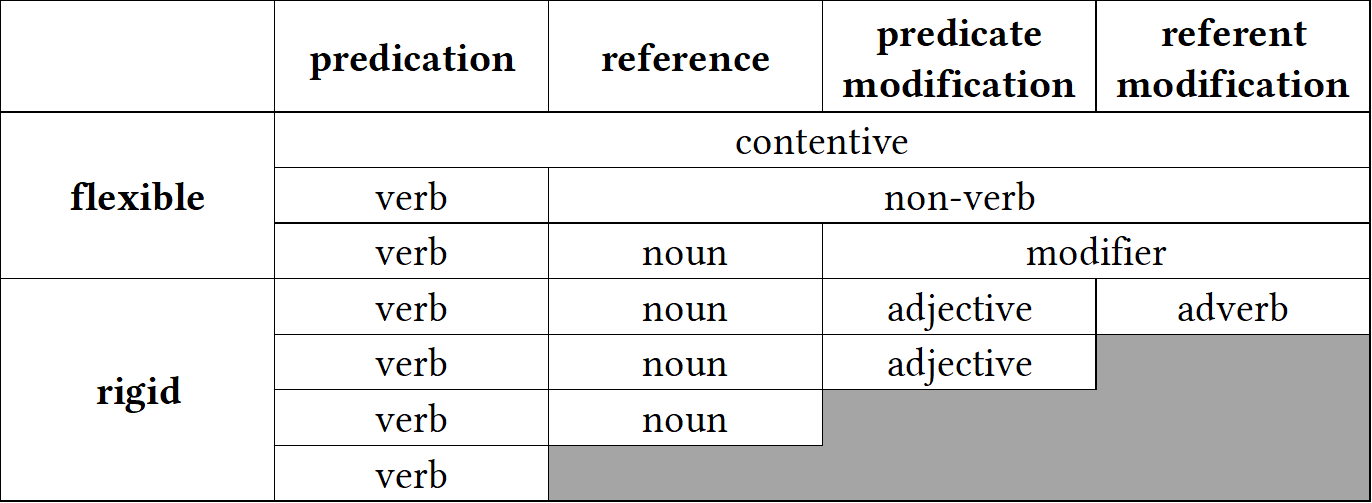
\includegraphics[width=\linewidth]{pos-typology.png}
  \caption[Hengeveld's typology of parts-of-speech systems]{\citeauthor{Hengeveld1992}'s \parencite*[69]{Hengeveld1992} typology of parts-of-speech systems}
  \label{fig:Hengeveld-post-systems}
\end{figure}

As mentioned in \secref*{sec:2.3.1.1}, \citeauthor{Hengeveld1992}'s typology could be criticized for its reliance on large, language-specific lexical categories instead of constructions. One could however reframe \citeauthor{Hengeveld1992}'s implicational hierarchy in terms of functions rather than catgories, as in \exref{ex:2.9}. I call this the \dfn{hierarchy of discourse functions}.

\begin{exe}
  \ex\label{ex:2.9} predicate > referent > predicate modifier > referent modifier
\end{exe}

\noindent In \exref{ex:2.9}, functions to the left of the hierarchy are more likely to have dedicated morphosyntactic constructions than those to the right. This reformulation avoids a commitment to any language-particular categories while still capturing the important implicational trend observed by Hengeveld.

This hierarchy of discourse functions has proven to be a fairly robust finding in the literature on lexical flexibility, now supported by a number of subsequent studies \parencites{Rijkhoff1998}{Anward2000}{Rijkhoff2000}{Vogel2000}{Beck2002}{Rijkhoff2003}{HengeveldRijkhoffSiewierska2004}{Lier2006}{Hengeveld2007}{HengeveldLier2010}{HengeveldValstar2010}{Beck2013}{Bisang2013}{Hengeveld2013}.

\subsubsection{Reference-predication asymmetries}
\label{sec:2.3.2.2}

The hierarchy of discourse functions also hints at another important feature of lexical categories: there is something privileged about the predicating function. A survey of the literature on lexical flexibility reveals patterned asymmetries in the behavior of lexical items with regard to predication vs. reference, even in very flexible cases. For starters, while it is quite common for languages to freely allow object words to be used as predicates with no special marking, the reverse case is much less likely \textcite[745]{HopperThompson1984}. The functional expansion of a word's uses from predication into reference always seems to be more marked (or at least as marked) as the shift from a referring function to a predicating function.

This fact has been observed independently by numerous researchers. For example, \textcite[251]{Stevick1968} and \textcite[373--374]{Marchand1969} both observe that conversion from noun to verb in \idx{English} has always been more common than from verb to noun, and \textcite[98]{Kastovsky1996} points out that English does not even have a native noun > verb derivational suffix—any affixes of this type are borrowed from \idx{Romance} languages. \idx{Central Alaskan Yup'ik} is another example of a language with very many nominalizers but few verbalizers \parencite[158]{Mithun2017}.

Flexibility itself is frequently \dfn{unidirectional}, meaning that any object word many be used for predication, but that action words used for reference are marked \parencites[69]{Croft2001b}[§3.3]{EvansOsada2005}{Beck2013}. \textcite[44]{Nakayama2001} frames flexibility in \idx{Nuuchahnulth} in terms of a word's ability to predicate, reporting that \textquote{all inflectional stems are potentially predicative}, but the reverse is not true. Discussing \idx{Classical Nahuatl}, Launey \parencites*{Launey1994}{Launey2004} introduces the term \dfn{omnipredicativity} to describe languages in which all words are potentially predicative, but no corresponding term \dfn{omnireferentiality} has appeared in the literature. That said, languages which have undergone \dfn{insubordination} \parentext{in which subordinate, usually nominalized clauses are reanalyzed as main clauses, and the nominal inflectional marking of the subordinate clause is reinterpreted as verbal inflectional marking \parencites{Evans2007}{Mithun2008}{EvansWatanabe2016}} do exhibit noun-oriented flexibility in the sense that verbal inflection mirrors nominal inflection. This famously led to the claim that all words in Eskimo languages are fundamentally nominal in nature \parencite{Sadock1999}. However, cases of insubordination do not constitute counterexamples to the predicating tendency in language. Even in these languages, the use of action words for reference is still less marked than the use of object words for predication; this includes \idx{Eskimo}, as mentioned for \idx{Central Alaskan Yup'ik} above.

\textcite{Kastovsky1996} argues that this asymmetry arises from the fact that \textquote[{\cite[96]{Kastovsky1996}}]{deverbal nouns have a much more diversified semantics than denominal verbs}, meaning that the range of possible meanings for a deverbal noun (a noun derived from a verb) is significantly broader than for a denominal verb (a verb derived from a noun). Examining data from \idx{English}, \citeauthor{Kastovsky1996} shows that when an object word is used to predicate,its possible meanings are limited to combinations of \textsc{be}, \textsc{be like}, \textsc{be in}, \textsc{become}, \textsc{have}, \textsc{do}, \textsc{do with}, and \textsc{cause}. When an action word is used as a predicate, however, the range of meanings include any abstract representation of the event itself (an action nominalization), or any one of the arguments associated with the verb, which come in a variety of semantic roles.

A similar, cognitively-oriented explanation for reference-predication asymmetries is given by \textcite[745]{HopperThompson1984}:

\blockquote[{\cite[745]{HopperThompson1984}}]{[A] nominalization names an event taken as an entity; however, a \enquote{verbalization} does not name an \enquote{entity taken as an event}, but simply names an event associated with some entity. In other words, a nominalization still names an event, albeit one which is being referred to rather than reported on in the discourse; it is, accordingly, still in part a [verb], and not a enquote{bona fide} [noun]. However, a denominal [verb] no longer names an entity at all, and thus has no nominal \enquote{stains} to prevent its being a bona fide [verb].}

\textcite[746]{HopperThompson1984} analyze nominalizations as a kind of metaphor following \citeauthor[3a]{LakoffJohnson1980}, in which an abstract event is conceptualized as a concrete object. However, no such metaphor exists for verbalizations, explaining the asymmetry in the directionality of lexical flexibility.

\subsubsection{Locus of categoriality}
\label{sec:2.3.2.3}

The grammatical level at which a language exhibits flexibility—the root, the stem, or the fully-inflected word—differs from one language to the next. In some languages, roots are strongly associated with a particular discourse function, but stems are flexible; in other languages, the reverse is true. I refer to the linguistic level at which a language associates different discourse functions as its \dfn{locus of categoriality}. Some linguistic theories include a premise that the locus of categoriality in every language always sits at a certain level \parencites{HalleMarantz1994}{Baker2003}{Baker2015}{BooijAudring2018}{Siddiqi2018}, but the evidence from research on lexical flexibility gives strong empirical support to the position that locus of categoriality varies from language to language. In contrast, \textcite{BlaszczakKlimekJankowskaMigdalski2015} argue that category information is distributed across different levels of representation.

As one illustration of how flexibility depends on grammatical level, we have seen that roots in \idx{Central Alaskan Yup'ik} are generally categorical—except for 12\% of roots, they are typically strongly associated with just one discourse function, and derivational affixes select for roots of a particular category \parencite[162--167]{Mithun2017}. While many derived stems are also strictly associated with just one discourse function, a large but indeterminate number have both referential and predicative uses. Examples of such flexible stems have already been shown in \exref{ex:1.7} in \secref*{sec:1.1}. Fully-inflected words in Central Alaskan Yup'ik, however, never exhibit flexibility \parencite[6]{Mithun2019}. So Central Alaskan Yup'ik displays partial flexibility at the root and stem level but not the inflected word level.

As another example, in \idx{Mandinka} all stems are flexible. No Mandinka stem except for \txn{sǎa} \tln{die} is used in just one discourse function \parencite[46]{Creissels2017}. At the level of the inflected word, however, lexical items in Mandinka belong unambiguously to one category or another \parencite[37]{Creissels2017}. Mandinka therefore shows complete flexibility at the stem level but complete rigidity at the inflected word level. (\citeauthor{Creissels2017} does not include an analysis of roots in his discussion.)

Surprisingly, some languages display flexibility even at the level of the fully-inflected word. In many North American languages, it is common for fully morphological verbs to function as referents \parencite{Hieberfc}, as shown in the following examples.

\begin{exe}

  \ex\label{ex:2.10}
  \exinfo{\idx{Chitimacha} (isolate)}
  \begin{xlist}

    \ex
    \glll dzampuyna\\
          dza‑ma‑(p)uy‑na\\
          thrust‑\gl{plact}‑\gl{hab}‑\gl{nf.pl}\\
    \tln{they usually thrust / spear with it}\\
    \tln{spear}
    \exsource[56]{Swadesh1939a}

    \ex
    \glll pamtuyna\\
          pamte‑(p)uy‑na\\
          ford‑\gl{hab}‑\gl{nf.pl}\\
    \tln{they usually cross (it)}\\
    \tln{bridge}
    \exsource[17]{Swadesh1939a}

  \end{xlist}

  \ex\label{ex:2.11}
  \exinfo{\idx{Cayuga} (Iroquoian > Lake Iroquoian)}
  \begin{xlist}

    \ex\label{ex:2.11a}
    \glll ǫtekhǫnyáʔthaʔ\\
          ye‑ate‑khw‑ǫni‑aʔt‑haʔ\\
          \gl{indef.agt.refl}‑meal‑make‑\gl{instr}‑\gl{ipfv}\\
    \tln{one makes a meal with it}\\
    \tln{restaurant}
    \exsource[200]{Mithun2000}

    \ex\label{ex:2.11b}
    \glll kaǫtanéhkwih\\
          ka‑rǫt‑a‑nehkwi\\
          \gl{neut.agt}‑log‑\gl{ep}‑haul.\gl{ipfv}\\
    \tln{it hauls logs}\\
    \tln{horse}
    \exsource[200]{Mithun2000}

  \end{xlist}

  \ex\label{ex:2.12}
  \exinfo{\idx{Navajo} (Na-Dene)}
  \begin{xlist}

    \ex
    \gll tsinaaʼeeɬ\\
         tsi(n)‑naaʼeeɬ\\
         wood‑it.moves.about.floating\\
    \tln{ship, boat}
    \exsource[316]{Young1989}

    \ex
    \gll chahaɬheeɬ\\
         it.is.dark\\
    \tln{darkness}
    \exsource[316]{Young1989}

  \end{xlist}

\end{exe}

\noindent Each of these flexible uses of a morphological verb sits somewhere on a continuum between being fully lexicalized as a referent, so that its predicating use is no longer available, to being a fully productive predicate, with both predicative and referential uses \parencite[413]{Mithun2000}.

The reason that words may exhibit flexibility at one level of analysis but not another is because \textquote[{\cite[1]{Mithun2019}}]{\emph{categorial} shift is often not \emph{categorical}}. When a word expands its use into new contexts, not all the morphological, syntactic, and semantic properties of the word shift to accommodate that new use at the same time. It takes some time before the morphosyntactic properties of a word adjust to reflect its new use, a process referred to as \dfn{actualization} in the grammaticalization literature \parencite{DeSmet2012} and \dfn{post-constructionalization constructional changes} in the framework of diachronic construction grammar \parencite[27]{HopperTraugott2003}.

It is because the locus of categoriality can vary from language to language that I have used the vague and overloaded terms \dfn{word} and \dfn{lexical item} throughout this thesis. Both are intended to be convenient cover terms for root, stem, or inflected word.

\subsubsection{Item-specificity}
\label{sec:2.3.2.4}

A final significant finding to emerge from the empirical research on lexical flexibility is the fact that flexibility is item-specific and even sense-specific. Individual lexical items or even individual senses of an item differ in their flexibility. To say that lexical flexibility is \dfn{item-specific} is to say that two words that are otherwise very similar in their meanings and morphosyntactic behavior can nonetheless differ in terms of their flexibility.

This fact is very nicely illustrated by both \citeauthor{Mithun2017}'s study of lexical flexibility in \idx{Central Alaskan Yup'ik} and \citeauthor{Creissels2017}'s study of \idx{Mandinka}. \textcite[163--164]{Mithun2017}, for example, considers roots for meteorological concepts, and shows that even within this small semantic domain, roots vary as to whether they exhibit flexibility. In \exref{ex:2.13a} the meteorological roots have predicative counterparts but in \exref{ex:2.13b} the meteorological roots do not.

\begin{exe}
  \ex\label{ex:2.13}
  \exinfo{\idx{Central Alaskan Yup'ik} (Eskimo-Aleut > Yupik)}
  \begin{xlist}

    \ex\label{ex:2.13a}
    \begin{tabularx}{\linewidth}[t]{ p{0.75in} >{\raggedright\arraybackslash\hangindent=1.5em}X p{1em} p{0.75in} >{\raggedright\arraybackslash\hangindent=1.5em}X }
      \txn{amirlu} & \tln{cloud}          & { } & \txn{amirlu‑} & \tln{be cloudy}\\
      \txn{kaneq}  & \tln{frost}          & { } & \txn{kaner‑}  & \tln{be frosted}\\
      \txn{aniu}   & \tln{snow on ground} & { } & \txn{aniu‑}   & \tln{to snow}\\
    \end{tabularx}

    \ex\label{ex:2.13b}
    \begin{tabularx}{\linewidth}[t]{ p{0.75in} >{\raggedright\arraybackslash\hangindent=1.5em}X p{1em} p{0.75in} >{\raggedright\arraybackslash\hangindent=1.5em}X }
      \txn{taituk}    & \tln{fog, mist} & { } & *\txn{taitug‑}    & \tln{be foggy}\\
      \txn{kavtak}    & \tln{hailstone} & { } & *\txn{kavtag‑}    & \tln{to hail}\\
      \txn{mecaliqaq} & \tln{sleet}     & { } & *\txn{mecaliqar‑} & \tln{to sleet}\\
    \end{tabularx}

  \end{xlist}
  \exsourcebelow[163]{Mithun2017}
\end{exe}

\noindent \citeauthor{Mithun2017} also provides similar data illustrating flexibility gaps for the domains of clothing and instruments:

\begin{exe}

  \ex\label{ex:2.14}
  \exinfo{\idx{Central Alaskan Yup'ik} (Eskimo-Aleut > Yupik)}
  \begin{xlist}

    \ex
    \begin{tabularx}{\linewidth}[t]{ p{0.75in} >{\raggedright\arraybackslash\hangindent=1.5em}X p{1em} p{0.75in} >{\raggedright\arraybackslash\hangindent=1.5em}X }
      \txn{taqmak} & \tln{dress}                & { } & \txn{taqmag‑} & \tln{put on a dress}\\
      \txn{nacaq}  & \tln{hat, parka hood, cap} & { } & \txn{nacar‑}  & \tln{put on a hat, hood}\\
      \txn{atkuk}  & \tln{parka}                & { } & \txn{atkug‑}  & \tln{put on a parka}\\
    \end{tabularx}

    \ex
    \begin{tabularx}{\linewidth}[t]{ p{0.75in} >{\raggedright\arraybackslash\hangindent=1.5em}X p{1em} p{0.75in} >{\raggedright\arraybackslash\hangindent=1.5em}X }
      *\txn{piluk} & \tln{footwear} & { } & \txn{pilug‑} & \tln{put on footwear}\\
      *\txn{at'e}  & \tln{clothing} & { } & \txn{at'e‑}  & \tln{don, put on clothing}\\
      *\txn{kive}  & \tln{pants}    & { } & \txn{kive‑}  & \tln{pull down pants}\\
    \end{tabularx}

  \end{xlist}

  \ex\label{ex:2.15}
  \exinfo{\idx{Central Alaskan Yup'ik} (Eskimo-Aleut > Yupik)}
  \begin{xlist}

    \ex
    \begin{tabularx}{\linewidth}[t]{ p{0.75in} >{\raggedright\arraybackslash\hangindent=1.5em}X p{1em} p{0.75in} >{\raggedright\arraybackslash\hangindent=1.5em}X }
      \txn{ay'uytaq}  & \tln{hockey stick}        & { } & \txn{ay'utar‑}   & \tln{play hockey}\\
      \txn{iqsak}     & \tln{fishhook}            & { } & \txn{iqsag‑}     & \tln{to jig for fish}\\
      \txn{kapkaanaq} & \tln{trap}                & { } & \txn{kapkaanar‑} & \tln{to trap, get trapped}\\
      \txn{keviq}     & \tln{plug, cork, stopper} & { } & \txn{kevir‑}     & \tln{to plug, stuff, caulk}\\
      \txn{kuvya}     & \tln{fishnet}             & { } & \txn{kuvya‑}     & \tln{fish by driftnetting}\\
    \end{tabularx}

    \ex
    \begin{tabularx}{\linewidth}[t]{ p{0.75in} >{\raggedright\arraybackslash\hangindent=1.5em}X p{1em} p{0.75in} >{\raggedright\arraybackslash\hangindent=1.5em}X }
      *\txn{kagi}   & \tln{broom}                & { } & \txn{kagi‑}   & \tln{sweep}\\
      *\txn{ipuk}   & \tln{ladle}                & { } & \txn{ipug‑}   & \tln{ladle, move with bow of boat high in air}\\
      *\txn{pangeq} & \tln{double-bladed paddle} & { } & \txn{panger-} & \tln{paddle with a double-bladed paddle}\\
    \end{tabularx}

  \end{xlist}

\end{exe}

\noindent On the basis of data like these, \citeauthor{Mithun2017} observes, \textquote[{\cite[163]{Mithun2017}}]{Speakers simply know whether a given root functions as a noun and what its meaning is, and whether it functions as a verb and what its meaning is. Gaps are not predictable[.]}. These gaps also vary from dialect to dialect. While the dialect in the above examples has no predicative counterpart for \txn{taituk} \tln{fog}, the Nunivak Island dialect has a pair of roots \txn{nugu} \tln{fog} and \txn{nungu-} \tln{be foggy}.

\citeauthor{Creissels2017}'s \parencite*{Creissels2017} study of \idx{Mandinka} is another good illustration of the item-specific nature of flexibility. While Mandinka has nominal and verbal constructions that allow the predicative and referring functions of words to be distinguished unambiguously, it is not as easy to separate word stems themselves into similar classes. In Mandinka, all items are flexible, but the \emph{way} in which items are flexible varies. Stems in Mandinka may be divided into three classes on the basis of their semantic behavior with regards to flexibility:

\begin{itemize}
  \singlespacing
  \item \textit{verbal} lexemes are those whose meaning is predictable when used to refer and therefore analyzable as a case of \enquote{morphologically unmarked nominalization}; these are always event nominalizations
  \item \textit{verbo-nominal} lexemes are those whose meaning in referring constructions is idiosyncratic and therefore not predictable
  \item \textit{nominal} lexemes are those whose meaning when used as predicates is predictable and limited to \tln{provide someone with X}
\end{itemize}

\noindent In \idx{Mandinka}, therefore, flexibility must be considered on an item-by-item basis, since the behavior of each item with regard to flexibility may differ.

In fact, flexible behavior in \idx{Mandinka} is not just item-specific, but sense-specific as well. \textcite[54]{Creissels2017} reports that polysemous lexemes may show different behavior for their different senses. The word \txn{díŋ}, for example, has two senses: \tln{child, young (of an animal)} and \tln{fruit}. However, only the \tln{fruit} sense is available for predication; when used as an intransitive verb, \txn{díŋ} may only mean \tln{bear fruit}, not \tln{give birth}, even though \tln{give birth} is a perfectly conceivable meaning of this word in predication. In the sense of \tln{child, young (of an animal)}, \txn{díŋ} behaves as a nominal lexeme, but in the sense of \tln{fruit} it behaves as a verbo-nominal lexeme. When lexical items undergo functional expansion into new discourse functions, it is also only specific senses that do so, not every sense of the word. More evidence for this comes from the diachronic development of the word \txn{run} in English: though the word \txn{run} when used as a predicate has numerous senses, the earliest attestations of \txn{run} used referentially are by and large with just the sense of \tln{fast pedestrian motion} (the exceptions to this stemming from just one corpus file) \parencite[76]{Gries2006}. Other refential uses of \txn{run} did not develop until later.

The existence of dialectal differences for flexibility as well as the unpredictable meanings of lexical items when used in various discourse functions show that the development of flexibility depends on conventionalization—whether a given form has assumed a conventionalized meaning in its role for a specific discourse function. These conventionalizations are language-specific, dialect-specific, item-specific, and even sense-specific \parencite[97]{Croft2000}. Speakers can and do playfully use existing lexical items for new discourse functions, but it is not until that combination of form and discourse function is conventionalized with a specific meaning in a community of speakers that we can say the word has undergone functional expansion. An excellent illustration of this is the word \txn{friend} in \idx{English}. Prior to the public availability of the social networking site Facebook in 2006, the use of \txn{friend} as a predicate had not been widely conventionalized. The growth of social networking then led to the very specific use of \txn{friend} to mean \tln{add as a connection on a social networking site}. Note that it does \emph{not} have the more general sense of \tln{be a friend} or \tln{befriend}. Like with Yup'ik\index{Central Alaskan Yup'ik} and \idx{Mandinka}, this shows not just that flexibility is item-specific, but that the meaning of flexible uses is often item-specific as well; in many cases it is unpredictable and must be memorized by speakers.

\subsection{Problems \& critiques}
\label{sec:2.3.3}

Despite the robust findings in \secref*{sec:2.3.2}, researchers have challenged the very possibility of lexical flexibility and its presence in various languages. Some of these challenges stem from the fact that certain conceptions of lexical flexibility are based on traditional ideas about the existence of large, language-specific parts of speech, and therefore subject to the same set of criticisms. Other challenges stem from precisely the facts presented in the previous section, especially that both flexibility and the meaning of flexible words are item-specific and often unpredictable, such that these words are not truly \enquote{flexible}. Moreover, languages must indicate the discourse function of their words \emph{somehow}—this is basic to our ability to communicate. So in a certain sense, the idea that there are words which are fully ambiguous as to their discourse function is doomed at the outset. The question is really where these indications of pragmatic function live—the root, the stem, the inflected word, or the clausal context. This section summarizes the main criticisms that scholars have raised against flexible analyses. In \secref*{sec:2.4}, we then look at alternative theories of word classes and their approach to lexical flexibility.

\subsubsection{Methodological opportunism}
\label{sec:2.3.3.1}

A methodological problem with certain theories of flexible words is that they, like traditional theories, commit the fallacy of \dfn{methodological opportunism} \parencite[30, 41]{Croft2001b} presented in \secref*{sec:2.2.3}. They do not apply the distributional method consistently. Instead, the criteria which separate words into categories are determined on the basis of additional theoretical commitments. \textcite[§2.2.2]{Croft2001b} criticizes Hengeveld's parts-of-speech typology on this basis, noting that Hengeveld ignores distributional evidence for classes smaller than the ones he posits in his typology (noun, contentive, etc.). \textcite{EvansOsada2005} raise similar concerns for Hengeveld's theory as applied to \idx{Mundari}. They state that in order for two lexical items to be members of the same lexical class, they must have \dfn{equivalent combinatorics}, which is to say that their distributions should be identical \parencite[366]{EvansOsada2005}. \citeauthor{EvansOsada2005} also state that in order for a language to flexible, that flexibility must be \dfn{exhaustive} in the sense that all members of a putatively flexible class must show equal degrees of flexibility and \dfn{bidirectional} in the sense that nouns may be used as verbs and vice versa. Both these criteria are merely different ways of reframing the broader principle that words in a class should share the same distributions \parencite[434]{Croft2005}. \citeauthor{EvansOsada2005} proceed to show various ways in which these criteria are not applicable to Mundari, and that Mundari is therefore not a flexible language. At the same time, however, \citeauthor{EvansOsada2005} use these facts to argue for the existence of the equally problematic categories of Noun and Verb in Mundari, using just a \textquote[{\cite[434, fn. 17]{EvansOsada2005}}]{canonical subset of distributional facts}. \citeauthor{Croft2005}'s \parencite*{Croft2005} commentary on \citeauthor{EvansOsada2005}'s target article is partially devoted to critiquing them on this point. The problem of methodological opportunism is present for any analysis which assumes that languages have a small set of large lexical categories—whether that analysis is flexible or traditional.

\subsubsection{Semantic shift}
\label{sec:2.3.3.2}

Broadly speaking, however, the primary argument against theories of flexible word classes is that they ignore a great deal of item-specific knowledge that speakers have about words and their uses in different functions \parencites[§3.2]{EvansOsada2005}[216]{Beck2013}. This issue has already been discussed in some detail in \secref*{sec:2.3.2.4}, but it bears explaining precisely why such item-specific knowledge constitutes a problem for theories of lexical flexibility.

For starters, when a lexical item expands into a new discourse function, there is a \dfn{semantic shift} in the direction of the meaning typically associated with the new context \parencites[74--77]{Croft1991}[73]{Croft2001b}. For example, when a property word is used in a referring expression, its meaning shifts to a person or thing with that property, not a reference to the abstract property itself. These semantic shifts cannot be attributed to some broader pragmatic principles—they are a matter of convention, and require broader uptake in a community of speakers in order to be conventionalized (as illustrated with the English word \txn{friend} above). Because the meaning that results from this semantic shift is conventional, often idiosyncratic, and language-specific, flexible words cannot be truly productive, as is implied by the term \enquote{flexible}. There is always a conventionalized component to their meanings.

Examples of idiosyncratic and unproductive shifts in the meaning of flexible words abound in the literature. Consider again the examples from \idx{Mundari} in \exref{ex:1.3}, repeated here as \exref{ex:2.16}.

\begin{exe}
  \ex\label{ex:2.16}
  \exinfo{\idx{Mundari} (Austroasiatic > Munda)}
  \begin{xlist}

    \ex
    \gll buru=ko                bai‑ke‑d‑a.\\
         mountain=\gl{3pl.subj} make‑\gl{compl}‑\gl{tr}‑\gl{ind}\\
    \tln{They made the mountain.}
    \exsource[354]{EvansOsada2005}

    \ex
    \gll saan=ko                buru‑ke‑d‑a.\\
         firewood=\gl{3pl.subj} mountain‑\gl{compl}‑\gl{tr}‑\gl{ind}\\
    \tln{They heaped up the firewood.}
    \exsource[355]{EvansOsada2005}

  \end{xlist}
\end{exe}

\noindent As a predicate, the stem \txn{buru} means \tln{heap up}, but this meaning is not predictable from just the combination of the nominal sense \tln{mountain} and its predicative use. The word could have just as easily meant \tln{climb a mountain} or \tln{overcome} or simply \tln{be a mountain}. No general pragmatic principles could have predicted this meaning. Likewise consider the \idx{Central Alaskan Yup'ik} examples from \exref{ex:1.7c}. Why does the combination of \txn{iqeq-} \tln{corner of mouth} + \txn{-mik} \tln{thing held in one's mouth}, \tln{to put in one's mouth} result in \txn{iqmik} \tln{chewing tobacco}? Why not \tln{oral thermometer} or \tln{toothpick}? Mithun provides many more unpredictable examples, shown in \exref{ex:2.17}.

\begin{exe}
  \ex\label{ex:2.17}
  \exinfo{\idx{Central Alaskan Yup'ik} (Eskimo-Aleut > Yupik)}
  \begin{xlist}

    \ex
    \begin{tabularx}{\linewidth}[t]{ p{1in} >{\raggedright\arraybackslash\hangindent=1.5em}X }
      \txn{mecur-} & \tln{get blood poisoning}\\
      \txn{mecuq}  & \tln{liquid part of something, sap, juice, green/waterlogged wood}\\
    \end{tabularx}

    \ex
    \begin{tabularx}{\linewidth}[t]{ p{1in} >{\raggedright\arraybackslash\hangindent=1.5em}X }
      \txn{melug-} & \tln{suck; eat roe directly from the fish}\\
      \txn{meluk}  & \tln{fish eggs, roe, fish eggs prepared by allowing them to age and become a sticky mess}\\
    \end{tabularx}

    \ex
    \begin{tabularx}{\linewidth}[t]{ p{1in} >{\raggedright\arraybackslash\hangindent=1.5em}X }
      \txn{qager-} & \tln{explode, to pop}\\
      \txn{qageq}  & \tln{blackfish which is boiled, allowed to set in its cooled, jelled broth}\\
    \end{tabularx}

    \ex
    \begin{tabularx}{\linewidth}[t]{ p{1in} >{\raggedright\arraybackslash\hangindent=1.5em}X }
      \txn{qumig-} & \tln{hold inside (of clothing)}\\
      \txn{qumik}  & \tln{enclosed thing, thing inside, fetus}\\
    \end{tabularx}

    \ex
    \begin{tabularx}{\linewidth}[t]{ p{1in} >{\raggedright\arraybackslash\hangindent=1.5em}X }
      \txn{aveg-} & \tln{divide in half, to halve}\\
      \txn{avek}  & \tln{half}; also \tln{half-dollar; person who is half Native}\\
    \end{tabularx}

    \ex
    \begin{tabularx}{\linewidth}[t]{ p{1in} >{\raggedright\arraybackslash\hangindent=1.5em}X }
      \txn{napa-} & \tln{stand upright}\\
      \txn{napa}  & \tln{tree}\\
    \end{tabularx}

    \ex
    \begin{tabularx}{\linewidth}[t]{ p{1in} >{\raggedright\arraybackslash\hangindent=1.5em}X }
      \txn{yuurqar-} & \tln{sip}\\
      \txn{yuurqaq}  & \tln{hot beverage, tea}\\
    \end{tabularx}

  \end{xlist}
\end{exe}

\noindent Or consider the example from \idx{Cayuga} in \exref{ex:2.11b}, repeated here as \exref{ex:2.18}.

\begin{exe}
  \ex\label{ex:2.18}
  \exinfo{\idx{Cayuga} (Iroquoian > Lake Iroquoian)}
  \glll kaǫtanéhkwih\\
        ka‑rǫt‑a‑nehkwi\\
        \gl{neut.agt}‑log‑\gl{ep}‑haul.\gl{ipfv}\\
  \tln{it hauls logs}\\
  \tln{horse}
  \exsource[200]{Mithun2000}
\end{exe}

\noindent Of all the possible nominal meanings that could reasonably derive from \tln{it hauls logs}—cart, tractor, ox—the fact that its nominal use means \tln{horse} is a fact specific to Cayuga that must merely be memorized by speakers.

Conventionalizations of lexical items used in new discourse functions also vary across languages. While the principle of semantic shifts still broadly holds, the specific meanings of these conventionalizations are unpredictable. Croft exemplifies this point by comparing \idx{English} \txn{school} with \idx{Tongan} \txn{ako} \tln{school / study}.

\blockquote[{\cite[71]{Croft2000}}]{English \txn{school} used predicatively does not mean the same thing as Tongan \txn{ako} used predicatively, namely \tln{study}. Going in the opposite direction, English \txn{study} used referentially does not mean the same thing as Tongan \txn{ako} used referentially, namely \tln{school}. Finally, English \txn{small} used referentially does not mean the same thing as Tongan \txn{si'i} \tln{childhood} used referentially.}

\noindent Since the meanings of putatively flexible words in different discourse functions are not predictable, many scholars reason that these words cannot be truly \enquote{flexible} in the sense of multifunctional or precategorial.

\subsubsection{Lexical gaps}
\label{sec:2.3.3.3}

Just as unpredictable in flexible cases is which sense of a word will be coopted into the new discourse function. In \idx{Wolof}, for example, the referential use of the word \txn{ndaw} can only mean \tln{young}, whereas the predicative use may mean either \tln{be young} or \tln{be little, small} \parencite[91]{Kihm2017}. We have also already seen similar lexical gaps for \idx{Central Alaskan Yup'ik} in \secref*{sec:2.3.2.4} above. If a lexical item lacks any conventionalized use in different discourse functions, than it cannot rightly be considered flexible, or a member of a flexible word class.

\subsubsection{Counterarguments}
\label{sec:2.3.3.4}

Pointing out that functional expansion involves both semantic shifts and functional gaps is generally intended to show that lexemes cannot be truly flexible in the sense of being multifunctional (\secref{sec:2.3.1.3}) or precategorial (\secref{sec:2.3.1.4}), and that uses of the same lexical item for different discourse functions should therefore be considered cases of conversion—that is, homonymy or heterosemy. There are however two major problems with this argument.

The first is that it creates a false dichotomy between homonymy and polysemy, when in fact the two phenomena are opposite endpoints on a continuum. Debates over the lexical unity of a word—that is, whether two uses of a lexical item are homonymous or polysemous—arise from an Aristotelian desire to neatly sort those uses into distinct lexemes, when in fact reality is much more complex. If this problem sounds familiar, that is because it is exactly the same methodological problem that arises when trying to exclusively categorize words into different classes. The complex adaptive nature of language makes categorical classification at either level impossible.

As discussed in \secref*{sec:2.3.1.4}, we know from cognitive research that mental categories are prototypal, and that the meanings of words display a polycentric, family resemblance structure. Two senses of a word are often related only tenuously through a network of intervening semantic connections or meaning chains. \textcite{Langacker1988} calls this the \dfn{network model} of category structure. \citeauthor{Taylor2003} points out that \textquote[{\cite[167]{Taylor2003}}]{[o]ne consequence of adopting the network model is that the question of whether a word is polysemous or not turns out to be incapable of receiving a definite answer.}

Over time, as this lexical network expands, the meanings of a word can diverge so drastically that speakers no longer have a direct cognitive association between them. \citeauthor{Mithun2000} exemplifies this nicely for both \idx{Cayuga} and \idx{English}. Discussing morphological Verbs used as referents in Cayuga, she notes the following:

\blockquote[{\cite[413]{Mithun2000}}]{If asked the meaning of \txn{kaǫtanéhkwih} [\tln{it hauls logs}], Cayuga speakers normally respond \tln{horse}. Though it has the morphological structure of a verb, it has been lexicalized as a nominal. The literal meanings of many verbal nominals are still accessible to speakers, but the origins of others have faded, and speakers express surprise at discovering them. Similarly, when asked \enquote{What would you like for breakfast?}, most English speakers do not think about breaking their night-time fast, though they can usually be made aware of the literal meaning of \txn{breakfast}.}

\noindent Lexicalization is a process and a continuum. Words can be lexicalized in new discourse functions to varying degrees. The first use of a lexical item in a new discourse function is innovative; each subsequent use then contributes further to its conventionalization.

Pointing out that functional expansion often creates idiosyncratic and unpredictable meanings essentially amounts to saying that senses of words can be highly divergent. This point is not in itself an argument against flexible analyses. Flexible words themselves may sit anywhere on the continuum from having closely connected, productive and predictable meanings, to having extremely divergent, idiosyncratic and unpredictable meanings. This is not a special fact about flexible words; it is simply true of words generally.

\textcite[73]{Croft2001b} expresses concern that ignoring semantic shifts in the analysis of flexible words overlooks important insights about how such semantic shifts are patterned (specifically, the universal fact that semantic shifts are always in the direction of the word's new discourse function). Given that so many researchers have indeed ignored semantic shift when arguing for flexible analyses, Croft's concern is warranted. However, it is entirely possible to define lexical flexibility in a way that both allows for the meaning of a lexical item to encompass multiple discourse functions and acknowledges that such multifunctional uses of the word involved patterned semantic shifts. The way to do this is to ground the definition of lexical flexibility in the pragmatic functions of reference, predication, and modification reather than language-specific categories like Noun, Verb, and Adjective. I offer such a definition in \secref*{sec:2.5}.

The second significant problem with using semantic shifts as an argument against the existence of flexible lexemes is that it proves too much. If semantic shift is taken as evidence against the lexical unity of putatively flexible words, then it must also be taken as evidence against the lexical unity of non-flexible words. Put simply, semantic shift is an analytical problem for all words, not just flexible ones.

This fact becomes clear when we ask, \enquote{What counts as a semantic shift? Just how \enquote{large} of a change in meaning (if it were even possible to quantify such a thing) does a semantic shift require?} To illustrate this problem, consider the semantic contribution of plural marking crosslinguistically. In the canonical case, plural marking is considered inflectional rather than derivational \parencite[2]{Corbett2000}, meaning that it does not create a new lexeme. Instead, it modifies the meaning of the existing lexeme slightly, in line with the classic distinction between inflection vs. derivation. However, there are numerous cases of words in English with more or less drastic differences in meaning between the singular and plural, and/or senses that are only available in one of the two numbers. Consider the examples in \exref{ex:2.19}.

\begin{exe}
  \ex\label{ex:2.19}
  \exinfo{\idx{English} (Indo-European > Germanic)}
  \begin{xlist}

    \ex
    \begin{tabular}[t]{ p{0.75in} l }
      \txn{air}  & \tln{atmosphere}\\
      \txn{airs} & \tln{affected manners}\\
    \end{tabular}

    \ex
    \begin{tabular}[t]{ p{0.75in} l }
      \txn{arm}  & \tln{upper limb; anything resembling a limb}\\
      \txn{arms} & \tln{weapons, firearms}\\
    \end{tabular}

    \ex
    \begin{tabular}[t]{ p{0.75in} l }
      \txn{blind}  & \tln{unable to see}\\
      \txn{blinds} & \tln{screen for a window}\\
    \end{tabular}

    \ex
    \begin{tabular}[t]{ p{0.75in} l }
      \txn{character}  & \tln{personality, mental qualities}\\
      \txn{characters} & \tln{people in a novel, play, or film}\\
    \end{tabular}

    \ex
    \begin{tabular}[t]{ p{0.75in} l }
      \txn{custom}  & \tln{tradition; socially accepted behavior}\\
      \txn{customs} & \tln{department which levies duties on imports}\\
    \end{tabular}

    \ex
    \begin{tabular}[t]{ p{0.75in} l }
      \txn{force}  & \tln{strength, energy}\\
      \txn{forces} & \tln{collection of military units}\\
    \end{tabular}

    \ex
    \begin{tabular}[t]{ p{0.75in} l }
      \txn{good}  & \tln{excellent, high quality}\\
      \txn{goods} & \tln{merchandise or possessions}\\
    \end{tabular}

    \ex
    \begin{tabular}[t]{ p{0.75in} l }
      \txn{manner}  & \tln{way of doing something}\\
      \txn{manners} & \tln{social conduct; socially acceptable conduct}\\
    \end{tabular}

    \ex
    \begin{tabular}[t]{ p{0.75in} l }
      \txn{spectacle}  & \tln{visually striking performance or display}\\
      \txn{spectacles} & \tln{pair of glasses}\\
    \end{tabular}

    \ex
    \begin{tabular}[t]{ p{0.75in} l }
      \txn{wood}  & \tln{fibrous material in the trunk of trees or shrubs}\\
      \txn{woods} & \tln{area of land covered with trees}\\
    \end{tabular}

  \end{xlist}
\end{exe}

Semantic shifts for plural marking in \idx{English} are not limited to just a handful of specific lexical items. Generic uses of the plural as in the expression \txn{foxes are cunning} create a semantic shift away from a concrete entity (\txn{a/the fox}) to a generic, unperceivable one—a use which strays from the prototypical function of nouns as concrete perceptible entities \parencite[708]{HopperThompson1984}.

As with flexible words, the semantic shifts that occur with plural marking can become so substantial that speakers no longer cognize the morphological singular and plural as members of the same word. Such is the case in the historical development of \txn{brother} vs. \txn{brethren} in \idx{English}. \txn{brethren} became so strongly conventionalized with its religious meaning in the plural that it was independently lexicalized as a plural-only (\foreign{plurale tantum}) noun, and the original plural underwent renewal with the emergence of the form \txn{brothers}. This is exactly the kind of lexicalization process that occurred for many morphological verbs reanalyzed as nouns in \idx{Cayuga} and many other North American languages.

A similar example comes from \idx{Chitimacha}, which has a pluractional marker \txn{-ma} indicating verbal number (plural agents, plural patients, or repeated action). In some cases the use of \txn{-ma} is purely compositional, so that it can be considered merely an inflectional marker of verbal number. In other cases \txn{-ma} so significantly alters the meaning of the word that it must be considered derivational. Compare the uses of \txn{-ma} in each of the pairs of verbs in \exref{ex:2.20} (note that \exref{ex:2.20b} and \exref{ex:2.20c} are phrasal verbs with a preverbal particle).

\begin{exe}
  \ex\label{ex:2.20}
  \exinfo{Chitimacha (isolate)}
  \begin{xlist}

    \ex\label{ex:2.20a}
    \begin{tabular}[t]{ p{1in} l }
        \txn{kow-}   & \tln{call}\\
        \txn{kooma-} & \tln{call multiple people}\\
    \end{tabular}

    \ex\label{ex:2.20b}
    \begin{tabular}[t]{ p{1in} l }
        \txn{qapx cuw-}   & \tln{come back; go about}\\
        \txn{qapx cuuma-} & \tln{travel; wander}\\
    \end{tabular}

    \ex\label{ex:2.20c}
    \begin{tabular}[t]{ p{1in} l }
        \txn{qapx qiy-}   & \tln{turn together; mix, join}\\
        \txn{qapx qiima-} & \tln{give a prayer, benediction; perform magic}\\
    \end{tabular}

  \end{xlist}
  \exsourcebelow{Swadesh1939a}
\end{exe}

\noindent In \exref{ex:2.20a}, the use of \txn{-ma} is entirely compositional. The presence of \txn{-ma} indicates that the verb has a plural patient argument. In \exref{ex:2.20b}, the use of \txn{-ma} is still arguably compositional, though perhaps somewhat lexicalized given the high frequency with which the word appears in the texts. \tln{travel, wander} could reasonably be interpreted as a continued repetition of \tln{go about}. In \exref{ex:2.20c}, however, \txn{qapx qiima-} has become lexicalized with a new meaning not directly related to that of \txn{qapx qiy-}. The diachronic connection between the two meanings is that prayers and magical incantations were traditionally accompanied by circling gestures with the arms. \txn{qapx qiima-} originally meant \tln{turn/circle around repeatedly}, but over time lexicalized with its new religious meaning in the pluractional, \tln{give a prayer, benediction}. This lexicalization process parallels that of \txn{brethren} in \idx{English}. Such a range of inflectional vs. derivational uses of pluractionals is quite common crosslinguistically \parencites{Mithun1988}{Mattiola2020}.

Finally, there are many languages which do not typically mark plurality on nouns \parencite{Dryer2013}, and yet have senses available in semantically plural contexts but not singular ones (where the semantic number can be understood from the clausal context, usually through verbal number marking). For example, the word \txn{soq} in \idx{Chitimacha} may mean \tln{foot} or \tln{paw} in a singular context and \tln{feet} or \tln{paws} in a plural context, but may also mean \tln{tracks} (e.g. animal tracks) in a plural context—a fairly significant and idiosyncratic shift in meaning, and one that is both language- and item-specific and thus conventional. This use constitues a \emph{morphologically unmarked semantic shift} in the meaning of the word, just as idiosyncratic meanings of words in cases of functional expansion also constitute morphologically unmarked semantic shifts. If we take such unmarked semantic shifts as evidence against lexical unity in the cases of flexible words, then we must also say that the \tln{foot} and \tln{tracks} meanings of \txn{soq} constitute two distinct lexemes as well.

One might ask, if we start splitting up lexemes based on every degree of semantic shift, where does the splitting stop? This is exactly analogous to the problem of lumping vs. splitting in the context of lexical categories. The Radical Construction Grammar solution to this problem is to abandon the commitment to larger groupings of items (the major lexical categories) and acknowledge that languages consist of an interconnected network of smaller items (constructions) instead \parencite{Croft2001b}. This approach has the major advantage of sidestepping unproductive debates about the existence or unity of particular lexical categories in particular languages, and shifts the focus instead to understanding the relationships and patterns among individual constructions. This is precisely what I propose to do for lexemes as well. If we abandon the idea that all the meanings associated with a form must be in some way grouped into lexemes based on their morphosyntactic contexts of occurrence, we sidestep unproductive debates regarding homonymy vs. polysemy, and can instead focus on the relationships and patterns among the various senses associated with that form—specifically, the nature of the semantic shifts that occur between uses of the form in different discourse functions.

In sum, idiosyncratic semantic shifts are not the problem for theories of lexical flexibility that they are often taken to be. Indeed, functional expansion wouldn't be possible if hearers weren't capable of determining the meaning of a form when used in even highly unusual contexts. Innovative uses of words in new functions would be all but impossible, providing no opportunity for such innovations to receive broader adoption in the linguistic community. Each time a hearer encounters a novel use of a lexical item for the first time, they must accomplish the difficult task of discerning its meaning. This is no less true for flexible words as it is for non-flexible words, or for words whose meaning is predictable vs. unpredictable. In a certain sense, \emph{every} use of a word is an instance of functional expansion, because every use of a word is always in a slightly different discourse and social context than the one before. The meaning of a word in a given context is highly socially and situationally dependent, and that context can change completely from one utterance to the next. Every token of a word thus necessarily appears in a new pragmatic context, and that pragmatic context slightly shapes its meaning. Language use is \emph{is} language change. Semantic shift is therefore an integral and ubiquitous part of language use; the question is simply the degree of that semantic shift.

\section{Functional approaches}
\label{sec:2.4}

By definition, functionalism as an approach to linguistic explanation is multifaceted. It looks to factors outside of the structural form of language as an explanation for that form—most especially cognition, usage effects from frequency, and information structuring in discourse \parencite[6323--6324]{Croft2001a}. A functional approach to lexical categories is one that utilizes these explanatory elements. In this section I present Croft's \parencites*{Croft1991}{Croft2000}{Croft2001b} functional theory of lexical categories, which explains crosslinguistic patterns in the coding of reference, predication, and modification as arising from the interaction between our mental categories and the needs of discourse. I then use this theory as a framework for defining lexical flexibility in \secref*{sec:2.5}. I begin with a brief discussion of prototype theory as it pertains to lexical categories (\secref{sec:2.4.1}), before expounding upon typological markedness theory (\secref{sec:2.4.2}).

\subsection{Prototype theory}
\label{sec:2.4.1}

It has long been recognized that the categories of human cognition are prototypal. In a series of studies, Eleanor Rosch and colleagues demonstrate that category membership is a matter of degree, and that there are better and worse representatives of any given mental category \parencites{Rosch1973a}{Rosch1973b}{Rosch1975}{RoschMervis1975}{Roschetal1976}{Rosch1978}. Prototype theory was then popularized in linguistics by \textcite{Lakoff1987}, \textcite{Langacker1987}, \citeauthor{Taylor2003} \parentext{[1989] \citeyear{Taylor2003}}, and Croft \parentext{[1990] \citeyear{Croft2003}; \citeyear{Croft1991}}, among others.

The evidence for prototype effects is robust \parencite[46--47]{Taylor2003}. When asked to rate whether an item is a good example of a category, participants consistently rate prototypical members are better examples of the category than non-prototypical ones. In listing experiments where participants are asked to list members of a category, prototypical members are listed earlier and more frequently than non-prototypical members. Finally, prototypical members of a category are identified by participants as being members of the category more quickly than non-prototypical members. Each of these effects is scalar, such that individual members of a category sit anywhere on a scale of more or less prototypical.

Linguistic constructions are also subject to prototype effects \parencite[Ch.~12]{Taylor2003}. \textcite{HopperThompson1980}, though not yet working in a prototype framework, nonetheless demonstrate that transitivity is very much a prototype category, with individual clauses showing greater or lesser degrees of transitivity depending on their features. \textcite{Ross1972} shows that lexical items are graded in their ability to undergo various transformations, with human beings being close to prototypical noun phrases, while inanimates, events, abstract concepts are quite atypical. \textcite[§12.5]{Taylor2003} likewise points out that the transitive construction in \idx{English} has steadily expanded its functions over time \textquote[{\cite[235]{Taylor2003}}]{to encode states of affairs which diverge increasingly from prototypical transitivity}. The result of this diachronic development is significant gradation as to which verbs now lend themselves to transitivization. \textcite[236]{Taylor2003} gives the example of the transitive construction being used to imply a semantic path, in lieu of an explicit preposition. Compare the pairs of \idx{English} sentences in \exref{ex:2.21}.

\begin{exe}
  \ex\label{ex:2.21}
  \hspace{0.5em}\exinfo{\idx{English} (Indo-European > Germanic)}\\
  \begin{tabular}[t]{ l l }
    \textit{Preposition}                         & \textit{Transitive}\\
    He regularly \em{flies across} the Atlantic. & He regularly \em{flies} the Atlantic.\\
    He \em{swam across} the Channel.             & He \em{swam} the Channel.\\
    She \em{swam across} our new swimming pool.  & ?She \em{swam} our new swimming pool.\\
    We \em{drove across} the Alps.               & ?We \em{drove} the Alps.\\
    The child \em{crawled across} the floor.     & *The child \em{crawled} the floor.\\
  \end{tabular}
  \vspace{0.5em}
  \exsourcebelow[236]{Taylor2003}
\end{exe}

\noindent These examples illustrate that there are indeed better and worse members of the \idx{English} Transitive Path construction.

Individual lexemes are also a type of construction, and therefore also subject to prototype effects. This is unsurprising since language forces speakers to map a non-discrete cognitive representation of the world onto discrete linguistic entities—we are forced to cut up and categorize the world around us into discrete objects and events/states so that we can refer to them and predicate statements about them. Reality, however, is not so neat. The result of this mapping is a linguistic form that imperfectly demarcates a portion of our mental world, centered on a clear prototype but with imprecise boundaries. Using a topological metaphor, we typically call some portion of our mental representation of the world a \dfn{semantic space} \parencites[140]{Finch2003}, and that space can be graphically represented using a \dfn{semantic map} \parencites[§2.4.3]{Croft2001b}{Haspelmath2003}. Though semantic maps are most often used to represent a \emph{functional} space for grammatical morphemes, they are equally applicable to lexical spaces as well. \textcite[74]{Gries2006} provides one such semantic map for the meanings of the \idx{English} word \txn{run}, shown in \figref{fig:semantic-map-run}, based on a comprehensive corpus analysis. \textcite[485]{BowermanChoi2001} present a semantic map of spatial relations on the basis of data from 38 languages (25 families), with a relation indicating prototypical support from below (\textsc{on}) at one end and a relation indicating prototypical containment (\textsc{in}) at the other. As pictured in \figref{fig:spatial-relations}, words in different languages cut up this semantic space in different ways.

\begin{landscape}
  \begin{figure}[h!]
    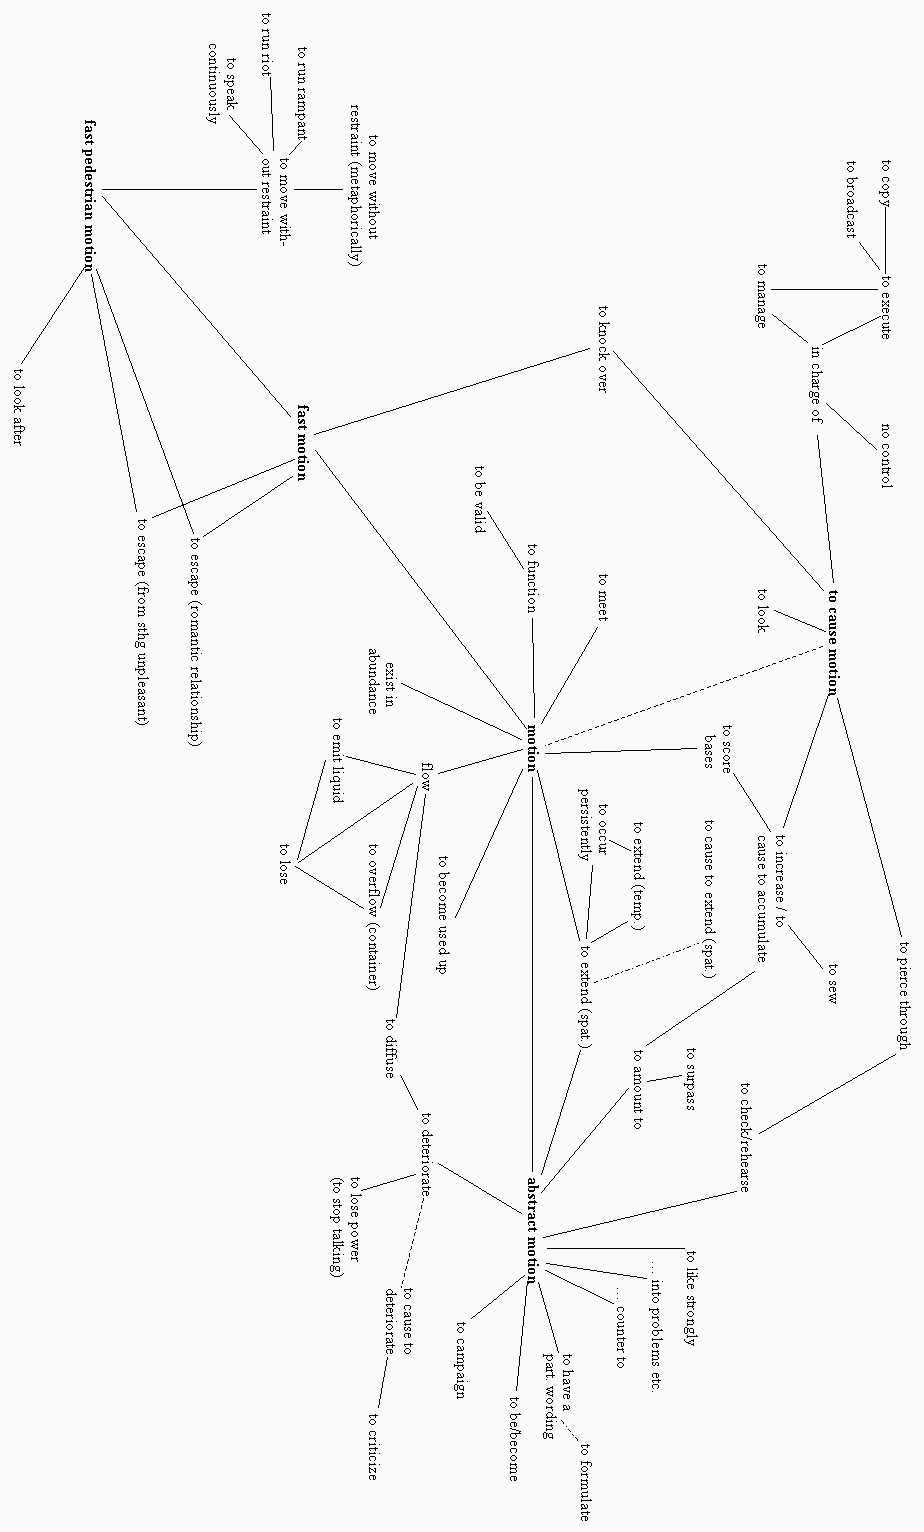
\includegraphics[width=\linewidth]{semantic-map-run.jpg}
    \caption[Semantic map of English \textit{run}]{Semantic map of \idx{English} \textit{run} \parencite[74]{Gries2006}}
    \label{fig:semantic-map-run}
  \end{figure}
\end{landscape}

\begin{figure}[h!]
  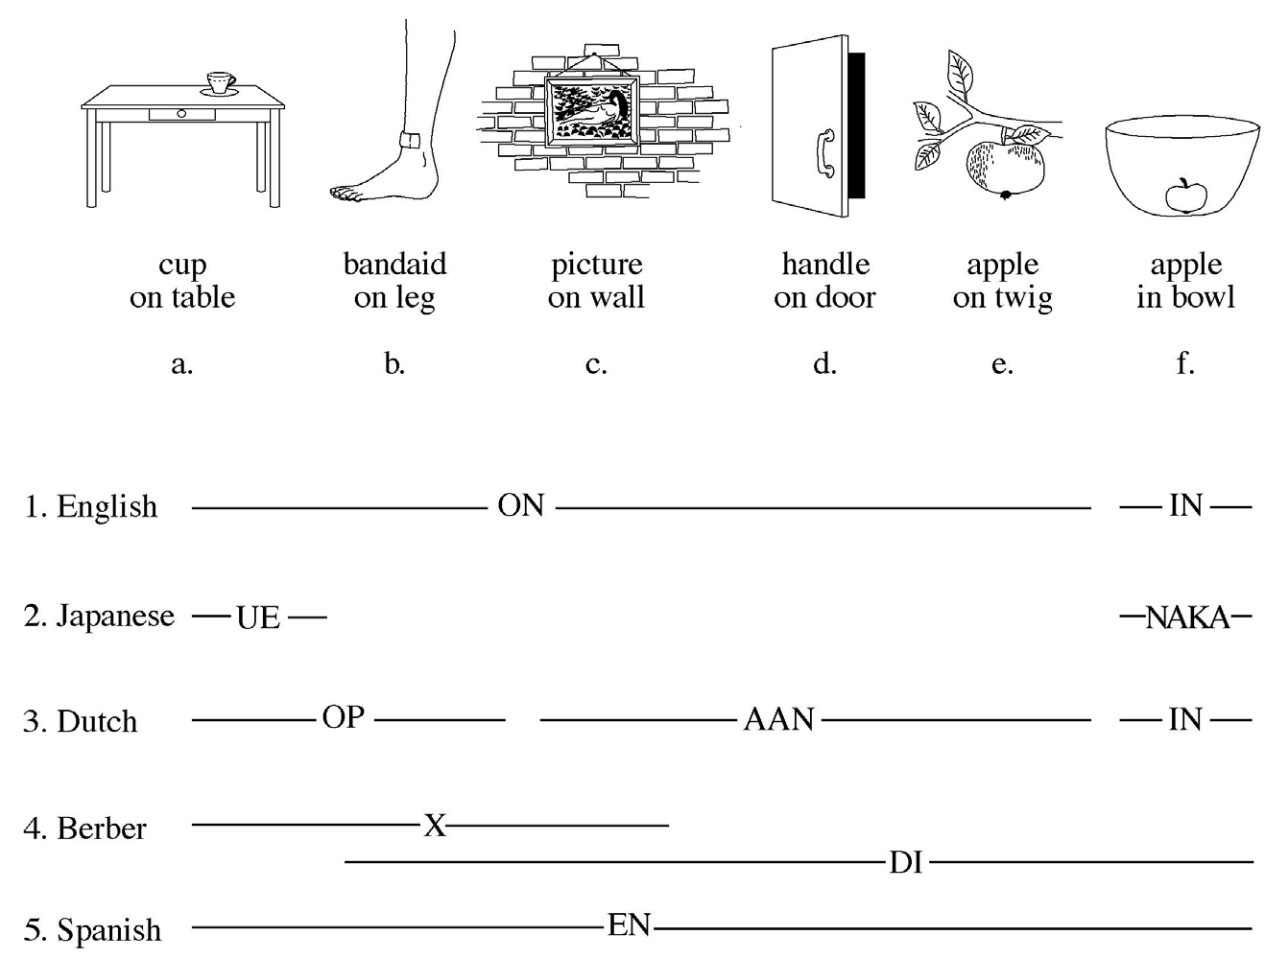
\includegraphics[width=\linewidth]{spatial-relations.jpg}
  \caption[Crosslinguistic differences in the encoding of spatial relationships]{Crosslinguistic differences in the encoding of spatial relationships \parencite[485]{BowermanChoi2001}}
  \label{fig:spatial-relations}
\end{figure}

These examples illustrate that word meanings are polycentric and cover a range of possible uses, as mentioned in \secref*{sec:2.3.1.4}. Some of these uses may be more prototypical than others. The \idx{English} expression \txn{apple on a twig} is a slightly less prototypical use of \txn{on} than \txn{apple on a table}. The fact that words cover a range of uses, and that some of these uses are more protoytpical than others, is an important component of the typological markedness theory of lexical categories.

Even the formal categories that linguists use to describe linguistic structure tend to be prototypal \parencite[xii, 201]{Taylor2003}. \textcite[§11.1]{Taylor2003} argues that linguists' conceptions of the formal labels \dfn{word}, \dfn{affix}, and \dfn{clitic} are prototypal in nature, with better and worse members of the category. \textcite{Haspelmath2005} likewise shows that simple structural definitions of these categories are inadequate, and reframes the word–affix continuum in functional terms instead. Much research in the Canonical Typology framework \parencite{Corbett2005} also demonstrates the prototypal nature of linguists' categories. Though Corbett is careful to distinguish between a \dfn{canon} and a \dfn{prototype} / \dfn{exemplar} \parencite[142]{Corbett2010}, his accumulated work nonetheless shows that linguists view phenomena in the world's languages as better or worse instances of various descriptive categories.

What type of category are lexical categories then? Are word classes categories of human cognition, categories within particular languages, categories of languages generally, or analytic categories of linguists? Or some combination of these? Typological markedness theory posits that parts of speech like noun, verb, and adjective are not categories of particular languages. Languages have constructions, not parts of speech. Speakers, however, have \emph{mental prototypes} of objects, actions, and properties. And although there is no \emph{singular} Noun construction in \idx{English} that would correspond to the mental category of \textsc{object}, there are numerous constructions in English which have the function of indicating \emph{reference to an object}, such as the Definite Article construction or the Transitive Subject construction. Likewise, there is no one construction—in English or any language—that can be definitively called the Verb construction or the Adjective construction, but there are plenty of constructions which have the function of predicating or attributing properties. Naturally, then, speakers are more likely to use referring constructions when talking about something which they mentally categorize as an object, predicating constructions when talking about something they conceive of as an action, and modifying constructions when talking about something they conceptualize as a property.

Speakers' conceptualizations, however, are fluid. Speakers often conceptualize things in non-prototypical ways. They may construe events as bounded entities that they can refer to, or objects as properties with duration. As a result, speakers often use words in constructions that do not align particularly well with the word's meaning, such as the appearance of an action word like \txn{sing} in a referring construction like the Gerund in the phrase \txn{his singing was beautiful}. When speakers use words in this atypical manner, those words are much more likely to be marked in some way—whether morphologically, behaviorally, semantically, or frequentiallyn \parencite[§2.2]{Croft1991}. As a consequence of this tendency, clear asymmetries emerge between the prototypical vs. non-prototypical uses of object words, action words, and property words. It is the unmarked use of these words that most closely aligns with linguists' traditional conceptions of noun, verb, and adjective. Parts of speech as traditionally conceived are nothing more than the emergent effects of our cognitive prototypes on language. They do not have any real status in grammar or individual grammars. This is the fundamental idea behind typological markedness theory. \secref*{sec:2.4.2} lays out this theory in more detail.

A last clarifying point is in order. Recognizing the existence of prototype-based categories, many linguists have described parts of speech as prototypal. \textcite[1--2]{Dixon2004}, for example, says that the word classes noun, verb, and adjective each have a \enquote{prototypical conceptual basis} and \enquote{prototypical grammatical functions}. \textcite[217]{Taylor2003} states, \enquote{A prototype view of \textsc{noun} entails that some nouns are better examples of the category, while others have a more marginal status.} But languages have constructions, not parts of speech, and individual constructions are not gradient \parencite{Croft2007}. What linguists are in fact observing when they say that parts of speech are prototypal is not gradation in \emph{linguistic categories} like noun, verb, and adjective (since those are not categories of particular languages), but rather gradation in the \emph{mental categories} of objects, actions, and properties, which do indeed exhibit prototype structures, and which therefore have emergent effects on the organization of constructions in languages.

\subsection{Typological markedness theory}
\label{sec:2.4.2}

I have already previewed various aspects of typological markedness theory at different points in this thesis. In this section I present a concise overview of the specific claims made by this theory, and some of the evidence for those claims. The phrase \dfn{typological markedness} or \dfn{typological markedness asymmetries} simply refers to an implicational universal regarding the behavior of basic versus non-basic members of a conceptual category. At its simplest, the theory posits that less basic or prototypical members of a category are marked in some way; basic or prototypical category members are unmarked by comparison \parencite{Greenberg1966}. This \emph{cognitive} markedness is then realized \emph{linguistically} in a number of ways. The marked member of a category \emph{may} be literally marked with some kind of affix or other overt morphological indicator, but this is just one of the ways an item can be a marked member of a category. The marked member of a category may also be less frequent, or have a smaller range of inflectional / distributional possibilities, or be semantically more complex. It is important to emphasize that \emph{typological} markedness does \emph{not} always entail \emph{formal} markedness. Typological markedness is an \dfn{implicational} universal rather than an \dfn{absolute} universal. The more marked members of a category must be \emph{at least as marked} as the unmarked member, but this does not preclude the possibility of all members being \emph{equally} marked. Formal markedness is merely an emergent tendency of structures to reflect cognitive markedness.

As applied to word classes, typological markedness theory states that the most unmarked discourse functions for object, action, and property words are reference, predication, and modification, respectively. Therefore, when a lexical item is used for a function that does not align with its prototypical meaning, typological markedness theory predicts that it will marked. Again, it must be emphasized that not \emph{every} instance of a lexical item being used in a non-prototypical function will be marked in comparison to its prototypical function; but it will always be \emph{at least as} marked. This theory of typological markedness for the major discourse functions is laid out in detail by Croft in various publications \parencites{Croft1991}{Croft2000}{Croft2001b}{CroftLier2012}. It is also important to understand that typological markedness theory is \emph{not} a theory of parts of speech in the sense of large partitionings of the lexicon into categories like noun, verb, and adjective. Instead, noun, verb, and adjective are epiphenomenal, crosslinguistic markedness patterns that arise from the interaction of semantic prototypes (object, action, property) and their use in different discourse functions (reference, predication, and modification). They are not categories of particular languages.

Throughout this thesis, I have used the term \dfn{discourse function} to refer to the functions of reference, predication, or modification. These are what \textcite[51]{Croft1991} calls \dfn{pragmatic functions} or \dfn{propositional act functions} following the tradition of pragmatics and speech act theory in philosophy \parencites{Austin1962}{Searle1976}. These three functions are taken as fundamental to human communication, arising out of the communicative intent behind what speakers are actually attempting to \emph{do} with language. This perspective was articulated early on by Sapir:

\blockquote[{\cite[87]{Sapir1921}}]{There must be something to talk about and something must be said about this subject of discourse once it is selected. This distinction is of such fundamental importance that the vast majority of languages have emphasized it by creating some sort of formal barrier between the two terms of the proposition.}

A similar point is made by Croft while articulating his theory of typological markedness as applied to lexical categories: \textquote[{\cite[124]{Croft1991}}]{[n]o matter how complex a given situation is in terms of the number of entities involved and the number and kinds of relations that hold between them, a human being attempting to describe it in natural language must split it into a series of reference-predication pairs[.]}

Modification is generally seen as less central a function than reference and predication, as illustrated by its lack of mention in the quotes above. For example, \textcite[55]{Hengeveld1992} takes the reference-predication dichotomy to be fundamental, yielding the major categories of noun and verb, while the modification function then combines with these two functions to yield the major categories of adjective and adverb, respectively. The primacy of the reference-predication distinction also appears to be reflected structurally in the world's languages, which do not always have dedicated means for encoding modification, but appear to always have constructions dedicated to reference and predication.

\textcite[123]{Croft1991} defines the pragmatic functions in terms of their discourse functions, following work in the discourse-functional tradition \parencites{Chafe1976}{HopperThompson1984}{Chafe1987}{DuBois1987}. Previous research defines \dfn{referents} as \textquote[{\cite[711]{HopperThompson1984}; \cite{Kibrik2011}}]{discourse-manipulable participants}, \dfn{predicates} as reported events \parencite[726]{HopperThompson1984}, and \dfn{modifiers} as a mix of these two functions \parencite{Thompson1989}. \textcite[123]{Croft1991} synthesizes ideas from this body of research and offers the following revised definitions instead:

\begin{itemize}
  \item the act of \dfn{reference} identifies a referent and establishes a cognitive file for that referent
  \item the act of \dfn{predication} ascribes something to a referent
  \item the act of \dfn{modification} enriches the cognitive image of the referent with an additional feature
\end{itemize}

\noindent The particular pragmatic function chosen for any given mention of a concept is then just a matter of how the speaker chooses to portray or construe that particular concept—whether as a referent, predicate, or modifier \parencite[100]{Croft1991}; as \citeauthor{CroftLier2012} note, \textquote[{\cite[63]{CroftLier2012}}]{apparent instances of \enquote{fuzziness} are actually variable construals}.

With this understanding of discourse functions in mind, we can restate the thesis of typological markedness theory as applied to lexical categories: Noun, verb, and adjective are epiphenomenal markedness patterns that arise from the use of different semantic prototypes (objects, actions, and properties) in different discourse functions (reference, predication, modification). Uses of these semantic classes in non-prototypical functions are typologically marked. As mentioned, there are four ways in non-prototypical uses can be marked: structurally, behaviorally, semantically, and/or frequentially.

The first type of marking, \dfn{structural coding} or \dfn{formal marking}, refers to the fact that non-prototypical uses of lexical items are at least as formally marked as prototypical ones. Structural coding in this context refers specifically to \textquote[{\cite[62]{CroftLier2012}}]{dedicated formal markers in a specific language that indicate a lexeme's syntactic function}. \figref{fig:typological-pos-prototypes} is a schematic representation of some of the formal realizations of these markedness patterns. In indicates the different morphosyntactic means that languages tend to develop for marking each of the non-prototypical uses of words. For instance, participle constructions are one way that languages have of indicating the non-prototypical case of an action word being used for modification.

\begin{figure}[h!]
  \centering
  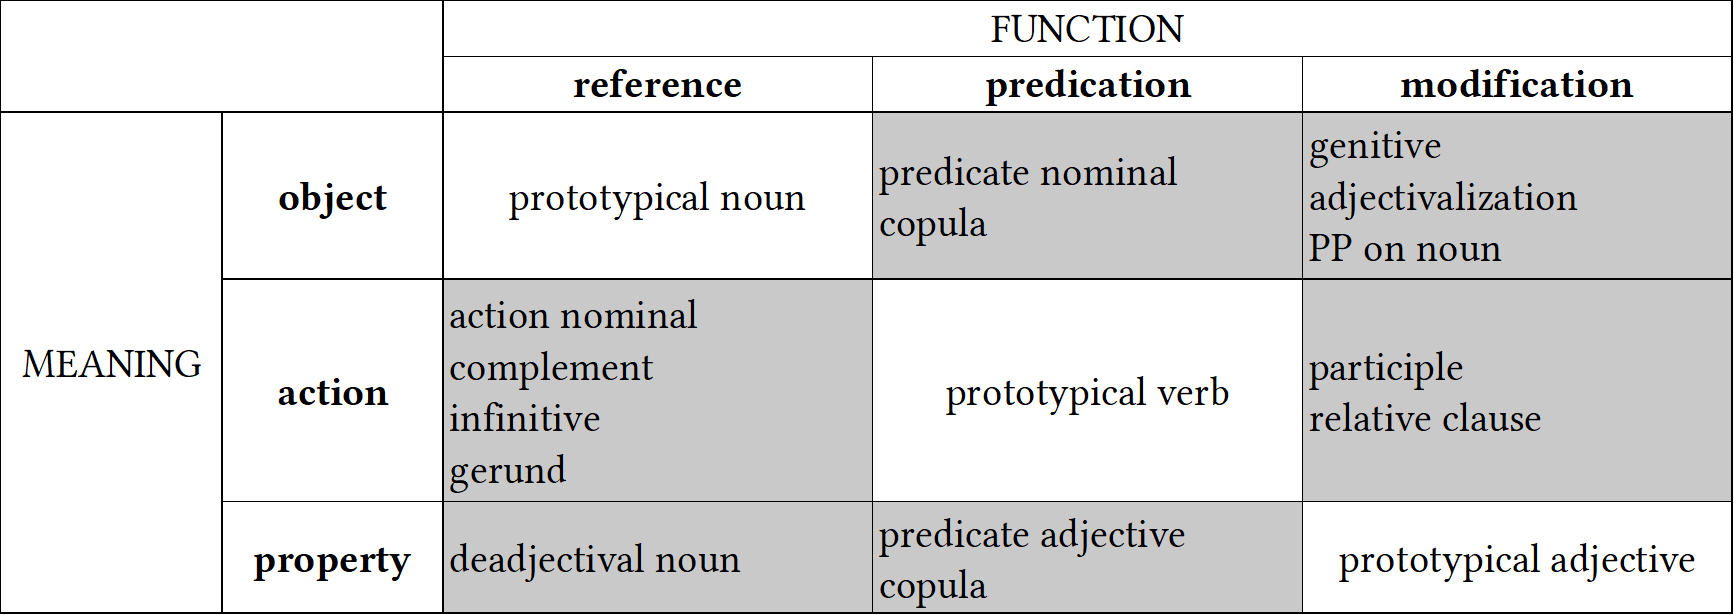
\includegraphics[width=\linewidth]{typological-pos-prototypes.png}
  \caption[Typological prototypes for noun, verb, and adjective]{Typological prototypes for noun, verb, and adjective (adapted from \textcite[89]{Croft2000} and \textcite[62]{Lier2012})}
  \label{fig:typological-pos-prototypes}
\end{figure}

The second way in which non-prototypical uses of words can be marked is in terms of their \dfn{behavioral potential}, that is, the range of combinatorial possibilities for that lexical item. This is most clearly illustrated with an example from inflection: in many languages, property words used in predicate constructions are limited in their inflectional possibilities. In \idx{Munya}, for example, property words functioning as predicates cannot inflect for person and number of the subject, and cannot take the imperfective marker, perfective marker, or direct evidential marker \parencite[96--97]{Bai2019}. The only grammatical markers allowed in property predication clauses are the stative aspect marker, a clause-final particle, and an egophoric marker. \citeauthor{HopperThompson1984}'s \parencite*{HopperThompson1984} study of the discourse functions of different parts of speech is largely a study of behavioral potential. They conclude that \textquote[{\cite[703, abstract]{HopperThompson1984}}]{the closer a form is to signaling this prime [prototypical] function, the more the language tends to recognize its function through morphemes typical of the category—e.g. deictic markers for [Nouns], tense markers for [Verbs].}. Croft advances a cognitive explanation for these behavioral markedness patterns:

\blockquote[{\cite[86]{Croft1991}}]{In general, only the core members of the syntactic category will display the full grammatical behavior characteristic of their category because only they have all the semantic characteristics that the characteristic inflections tap into. This is to say that the inflectional categories of the major syntactic categories have been \enquote{tailored} to their semantically core members. This is an example of a processing constraint: languages inflect only for those properties that are of relevance to core members of the category; they do not inflect for properties of peripheral members of the category that are not of relevance to the core members of the category.}

Non-prototypical uses of words may also be marked semantically by a \dfn{semantic shift} in their meaning towards the semantic class prototypically associated with the discourse function they are found in \parencites[96]{Croft2000}[73]{Croft2001b}[68]{CroftLier2012}. I have already discussed the semantic shifts that occur in functional expansion in some detail in \secref*{sec:2.3.3.2}. \textcite[60--61]{Croft1991} makes the even stronger claim that non-prototypical uses of words will \emph{always} be marked semantically, making semantic markedness an absolute rather than implicational universal.

These semantic shifts are caused by a combination of conventionalization and \dfn{coercion}, wherein the meaning of the construction is imposed on the meaning of the lexical item \parencite{Pustejovsky1991}[69, 108]{Croft1991}[252]{PantherThornburg2007}{AudringBooij2016}. For example, predicate nominals (wherein an object word is used in a predicate construction) involve coercion from denoting an object to denoting classifying or equational relations \parencite[69]{Croft1991}. In \idx{Nuuchahnulth}, for example, nominal predicates are always semantically durative and interpreted as either existential, classifying, or identifying expressions \parencite[47]{Nakayama2001}.

The final way in which words used in atypical functions may be marked is in terms of their frequency. \textcite[59, 87]{Croft1991} also refers to this as \dfn{textual markedness}. Frequential markedness predicts that lexical items are used more frequently in their prototypical functions than in non-prototypical ones. This means that object words should be most frequent in their use in referring constructions, and that referring constructions should most frequently denote objects \parencite[87]{Croft1991}.

The field of linguistics has accumulated a good deal of empirical evidence in support of the typological markedness theory of lexical categories. \textcite{Croft1991} provides empirical evidence from 12 languges for each of these markedness patterns. \textcite{Dixon1977} also provides evidence of typological markedness patterns as they relate to property words, using a combination of structural and behavioral evidence. As mentioned, \citeauthor{HopperThompson1984}'s \parencite*{HopperThompson1984} study also provides empirical support from a variety of languages for markedness in terms of behavioral potential. \textcite{Stassen1997} is a massive study of intransitive predication in 410 languages, demonstrating the marked behavior of non-action words when used in predicate constructions.

Having explicated the basic tenets of typological markedness theory, I now turn to reframing the concept of lexical flexibility in a way that utilizes this framework.

\section{Lexical flexibility: A functional definition}
\label{sec:2.5}

Within the framework of typological markedness asymmetries, lexical flexibility can be understood as follows:

\begin{description}
  \item[lexical flexibility] The use of a lexical item (root, stem, or inflected word) in more than one discourse function (reference, predication, or modification) with no difference in structural coding.
\end{description}

This definition qualifies as a valid \dfn{comparative concept} in the sense of \textcite{Haspelmath2010a}, because it is couched in terms of universal \emph{functions} rather than language-specific \emph{structures} \parencite{Croft2016}. It also has the advantage of being intentionally equivocal with respect to the lexical and cognitive unity of the item, and with respect to the linguistic level (root, stem, or inflected word) at which the flexibility is realized. In some cases when a single lexical form appears in more than one discourse function, speakers may have a close cognitive association between the two uses. This is most likely the case for the predicative and referential uses of the word \txn{run} in the phrases \txn{I run every morning} and \txn{I'm going for a run} respectively. In other cases, speakers may have little to no awareness of the diachronic connection between uses of a form. For example, the use of \txn{run} in the sense of \txn{to run a print job} is extremely distant from the prototypical \enquote{fast pedestrian motion} sense in the semantic network for that form \parentext{\cite[74]{Gries2006}; see also \figref{fig:semantic-map-run}}. It is unlikely that these two senses are closely cognitively connected by most speakers, despite the fact that they both share a predicating function. The definition of lexical flexibility given here allows for any degree of semantic shift. \citeauthor{Croft2001} admits of this possibility explicitly: \textquote[{\cite[68]{Croft2001b}}]{It of course a priori possible to construct a typological classification of parts-of-speech systems using only structural coding and allowing any degree of semantic shift.} Of course, I am not concerned here with constructing a classification of parts of speech—quite the opposite, in fact. This definition of lexical flexibility is intended to delimit precisely the cases where a language does \emph{not} provide formal indicators of discourse function.

Allowing for any degree of semantic shift does \emph{not} imply that semantic shift is in any way unimportant for understanding lexical flexibility. On the contrary, semantic shift is a key component of the process of functional expansion that leads to flexibility in the first place (see below). Moreover, carefully circumscribing the phenomenon of lexical flexibility without regard to the degree and type of semantic shifts involved puts us in a position to then compare the semantic shifts that occur in cases of lexical flexibility with those that occur in cases of overt derivation. This raises the intriguing question of whether semantic shifts in flexible cases differ in principled ways from overt derivation. \textcite[165]{Mithun2017} shows that for \idx{Central Alaskan Yup'ik} the types of semantic relationships between flexible uses of words mirror those between basic and derived words. This would suggest that functional expansion follows the same principles as overt derivation. However, much more research is needed in this area.

As we have seen, a great abundance of evidence also shows that the meaning of any given combination of form and discourse function is a matter of convention, and often highly idiosyncratic (\secref(sec:2.3.2.4); \secref{sec:2.3.3.2}). This fact suggests that flexible items are not truly \enquote{flexible} in the sense that speakers can use any lexical item for any discourse function and expect hearers to be able to infer their meaning from context. We know that item-specific gaps in usage exist. Certainly, novel cases of forms being used in new discourse functions do occur, or else it would not be possible for functional shift to happen in the first place. But these cases are necessarily restricted by the cognitive limits on our ability to deal with ambiguity. If it were truly the case that any lexical item could be used in any discourse function at any time, it would barely be possible for hearers to interpret the intended pragmatic effects of each word. Instead, flexibility must rely on a degree of \emph{conventionalization}. Conventionalization in turn implies \emph{time}—conventionalization is a diachronic process. Thus, \emph{lexical flexibility is best understood as a synchronic pattern resulting from the diachronic process of functional expansion}, where functional expansion is defined as follows:

\begin{description}
  \item[functional expansion] A diachronic expansion in the use of a lexical item (root, stem, or inflected word) into a new discourse function (reference, predication, or modification) with no additional structural coding.
\end{description}

\noindent Cases of lexical flexibility therefore arise whenever a new combination of form and discourse function is conventionalized in a community of speakers. This understanding of lexical flexibility is in line with cognitive research on lexicalization and constructional change. Functional expansion occurs because of speakers' need to construe concepts in different ways—as objects, actions, or properties. The semantic shifts that occur during functional expansion are then the result of coercion by the new constructional context, and the resultant meaning then becomes conventionalized as the meaning of that particular form in that particular discourse function \parencite[108]{Croft1991}.

If lexical flexibility is the result of a diachronic process, it should be possible to enumerate some of the specific pathways which give rise to it. Here I will mention just a few. One pathway is insubordination, whereby subordinate clauses in a language are reanalyzed as main clauses \parencites{Evans2007}{Mithun2008}{EvansWatanabe2016} (see also \secref{sec:2.3.2.2}). Insubordination frequently results in formal similarities between noun phrases and verb phrases, and this formal ambiguity can abet the functional expansion of lexical items from referential to predicative uses and vice versa.

A second pathway to lexical flexibility is relexicalization (or more precisely, reconventionalization). This is the process that occurred in the case of morphological verbs being reanalyzed as nouns in many North American languages (see \secref{sec:2.3.2.3}) and certain \idx{English} plurals like \txn{brethren} or \txn{arms}. In these cases, the conventionalized meaning associated with the form changed (e.g. from \idx{Cayuga} \tln{it hauls logs} to \tln{horse}), so that the meaning more closely reflected its new discourse context.

A third pathway is topicalization, exemplified in the \idx{Wakashan} family. \textcite[122, 142]{Jacobsen1979} observes the formal similarity between the Definite Article and the Third Person Singular Indicative markers in Wakashan languages, and argues for a diachronic connection between the two. It is likely that cleft constructions such as \tln{it was the dog that ran} became so common that speakers started to reanalyze the topicalized cleft as a definite noun phrase, \tln{the dog}, thereby creating a formal similarity between referring expressions and predicating expressions.

Each of these pathways results in the functional expansion of lexical items into new discourse contexts with no new overt structural coding. Of course, functional expansion can also occur without any other accompanying grammatical changes. This happens in any instance where speakers simply use stems in new discourse functions. Lexical flexibility is the natural and expected result of the fact that non-prototypical uses of words are \emph{not} always structurally marked—as allowed for by the fact that typological markedness is implicational and not absolute—even if they are marked in other ways. The use of additional structural coding in cases of functional expansion is not obligatory, but merely a statistical tendency. Lexical flexibility occupies the theoretical space where structural coding asymmetries fail to apply.

When viewed in this light, \emph{lexical flexibility is not so much of a problem as it is a design feature of language}. The presence of lexical flexibility should be \emph{expected} in every language, not treated as exotic. The cognitive-typological approach outlined in this chapter inverts the lexical flexibility question: the interesting question is not why some languages fail to make distinctions in parts of speech (thereby framing lexical flexibility as a \emph{deficit}), but rather why languages develop specialized constructions for different discourse functions in the first place \parentext{see \textcite{Gil2012} for an attempt to answer this question for predication}. Lexical flexibility exists in any area of the grammar where specialized function-indicating morphology has yet to develop. Flexibility should therefore be considered the default state of affairs for language. Gil \parencites*{Gil2005}{Gil2006} has in fact argued, partially on the basis of data from highly flexible languages, that early human language must have been \dfn{isolating-monocategorial-associational} before the development of dedicated function-indicating morphology.

The idea that the \enquote{natural state} of language is monocategorial or acategorial would seem to conflict with the point made above that lexical flexibility can result from diachronic processes, but the two positions are not mutually exclusive. Languages develop constructions which indicate different discourse functions, but languages are also subject to counteracting pressures. This is a classic case of competing motivations: on the one hand, the frequency with which speakers need to perform the discourse functions of reference, predication, and modification all but ensures the development of constructions dedicated to indicating those functions; on the other hand, speakers need to construe states of affairs in various ways—as objects, actions, or properties—creating pressures which have the potential to level those formally marked distinctions. Reconventionalization and the reanalysis of cleft constructions could both be viewed as diachronic processes motivated by this latter pressure.

In sum, then, lexical flexibility is a natural result of the cognitive and diachronic forces at work in language. Defining lexical flexibility in terms of typological markedness (or more accurately, the lack of formal marking for otherwise marked uses) provides a crosslinguistically applicable definition of the phenomenon which avoids methodological opportunism while still recognizing that lexical flexibility requires some degree of semantic shift and conventionalization. With this definition in place, the remainder of this thesis turns to exploring the prevalence of lexical flexibility in \idx{English} and \idx{Nuuchahnulth} and the semantic behavior of words in cases of functional expansion.
